
\documentclass[pdftex,a4paper,11pt,DIV15,BCOR20mm,parskip,numbers=noenddot]{scrbook}

% \usepackage{default}
\usepackage[ngerman]{babel} % Deutsche Formattierung
\usepackage[T1]{fontenc}
\usepackage[utf8]{inputenc} % Zeichenkodierung
\usepackage[pdftex]{color} % Farben
\usepackage{setspace} % Das Paket setspace ermöglicht ein einfaches Umstellen von normalem, anderthalbfachen oder doppeltem Zeilenabstand.
\usepackage[pdftex]{graphicx} % Bilder
\usepackage[final]{listings}  % ermöglicht die Darstellung von (Programm-)Quellcode in der Arbeit
\usepackage[normalem]{ulem} % ermöglicht das Unterstreichen von Text
\usepackage{amsfonts} % ok-zeichen usw
\usepackage{amsmath} % mathekrams
\usepackage{scrpage2}
\usepackage{babelbib} % Bibliographie
\usepackage{array} % für tabellen
\usepackage[style=base,margin=10pt,font=footnotesize,labelfont=bf]{caption} % Formattierung Bildunterschrift
\usepackage{listings} % Quellcode
\usepackage{float} % floating figures
\usepackage{tikz} % Diagramme
\usepackage{wrapfig} % Text neben Abbildungen
\usepackage{pdflscape} % Seiten in Querformat
\usepackage{geometry}
\usepackage{soul}
\usepackage{textcomp} % Quote Symbol
\usepackage{pifont}% http://ctan.org/pkg/pifont

\newcommand{\cmark}{\ding{51}}%
\newcommand{\xmark}{\ding{55}}%

% schrift auf palatino umstellen
\usepackage{palatino}
\setkomafont{sectioning}{\normalcolor\bfseries} 
% \renewcommand{\familydefault}{\sfdefault}

\definecolor{uhhred}{cmyk}{0,1,1,0}
\definecolor{beige}{RGB}{194,116,31}
\definecolor{green}{RGB}{41,128,38}
\definecolor{brown}{RGB}{132,60,36}
\definecolor{darkblue}{RGB}{38,38,128}

\newcommand{\routput}{\vspace{-0.25cm}\hspace{5pt}\small\color{blue}\ttfamily} 
\newcommand{\rsymbol}{\vspace{-0.25cm}\hspace{5pt}\small\color{blue}\ttfamily\textquotesingle}
\newcommand{\rerror}{\vspace{-0.25cm}\hspace{5pt}\small\color{red}\ttfamily$\bigotimes$ \hspace{0cm}}

\newcommand{\q}{\textquotesingle}
\newcommand{\qq}{\textquotedbl}
    
% Listing-Formattierung
\lstset{
    backgroundcolor=\color{white}, 		% white background
    %     columns=fullflexible, 			% allow latex to break lines
    numbers=none, 				% no line numbering
    showstringspaces=false, 			% no gap character in strings
    belowskip=-10pt, 				% remove blank space at the bottom of listing
    basicstyle=\ttfamily\small\color{darkblue}, 
    xleftmargin=5pt, % Padding
    language=Lisp, 				% for highliting comments and literals
    commentstyle=\color{beige}, 		% comment style
    stringstyle=\color{green}, 			% literal style
    numberstyle=\color{green},
    alsoletter={\#, >},
    keywordstyle=\ttfamily, 			% keyword style
    keywordstyle=[2]\color{green},		% style for literals
    keywordstyle=[3]\color{black},	% style for non-terminals
    literate=
	  *{(}{{{\color{brown}{(}}}}{1} 	% colored brackets
	  {)}{{{\color{brown}{)}}}}{1}	 	
	  {{[}}{{{\color{brown}{{[}}}}}{1}
	  {{]}}{{{\color{brown}{{]}}}}}{1}
	  {\{}{{{\color{brown}{\{}}}}{1}
	  {\}}{{{\color{brown}{\}}}}}{1}
	  {'}{{{\bfseries\color{green}{\textquotesingle}}}}{1}
	  {\#'}{{{\color{green}{\#\bfseries\textquotesingle}}}}{1}
	  {lambda}{{$\lambda$}}{1},
%     % lists of keywords
%     morekeywords={},
    keywords=[2]{\#t, \#f},
    keywords=[3]{\#lang swindle, \#lang racket, >} 
}

\makeatletter
\newcommand{\thickhline}{%
    \noalign {\ifnum 0=`}\fi \hrule height 1.2pt
    \futurelet \reserved@a \@xhline
}
\newcolumntype{'}{@{\hskip\tabcolsep\vrule width 1.2pt\hskip\tabcolsep}}
\makeatother
  
%   % Tikz styles
%   \usetikzlibrary{shapes,arrows,decorations.markings}
%   \tikzstyle{block} = [rectangle, draw, fill=gray!15, text width=11em, text centered, rounded corners, minimum height=3em]
%   \tikzstyle{label} = [text centered]
%   \tikzstyle{arrow} = [draw, -latex', thick, postaction={decorate}] 
%   \tikzstyle{line} = [draw, -, thick]
  
\usepackage{etoolbox}
\makeatletter
\patchcmd{\chapter}{\if@openright\cleardoublepage\else\clearpage\fi}{}{}{}
\makeatother  
	
\usepackage{colortbl} % für farbige Tabellen
\usepackage{longtable} % für mehrseitige Tabellen
\renewcommand{\arraystretch}{1.25} % in Tabellen: Padding des Textes nach oben und unten in Prozent

% Fußnoten werden im gesamten Dokument fortlaufend hochgezählt und nicht nur kapitelweise, vgl. http://www.golatex.de/nummerierung-der-fussnoten-durchgehend-im-gesamten-dokument-t2042.html
\usepackage{chngcntr}
\counterwithout{footnote}{chapter}

\setlength{\emergencystretch}{1em} % Für den Fall, dass Zeilen im 1. Anlauf nicht richtig umgebrochen werden können, einen 'Notfallraum' einrichten (vgl. http://www.golatex.de/overfull-boxes-in-latex-t1979.html) 

% entnommen aus http://www.siart.de/typografie/latextipps.xhtml#floats
\renewcommand{\floatpagefraction}{0.8} % gibt den Bruchteil einer Seite, die für Gleitobjekte benutzt wird, an, der erreicht werden muss, bevor eine neue Seite angefangen wird. (Standard: 0.5; d.h. wenn ein Bild 51% der Seite einnimmt, wird extra für dieses Bild eine ganze Seite reserviert --> unschön)
\renewcommand{\topfraction}      {0.8}
\renewcommand{\bottomfraction}   {0.5} % \topfraction / \bottomfraction, gibt den Bruchteil einer Seite an, bis zu dem Gleitobjekte oben bzw. unten angeordnet werden sollen.
\renewcommand{\textfraction}     {0.15} % gibt den Bruchteil einer Seite an, der mit Text belegt werden können muss.
\makeatletter
  \setlength{\@fptop}{0pt} % Wenn ein Float-Objekt allein auf einer Seite steht, soll es am oberen Rand der Seite erscheinen und nicht vertikal zentriert
\makeatother

  \usepackage[
%   	pdfstartview={Fit},   
%   	pdffitwindow=true,
  	colorlinks,
  	linkcolor=black,
  	anchorcolor=black,
  	citecolor=black,
  	urlcolor=black,
  	bookmarks, 
  ]{hyperref}
   
% Zeilenabstand
% \setstretch{1.24}   

% Strafpunkte, die beim Seitenumbruch vergeben werden, falls die erste Zeile eines Absatzes allein auf der vorangehenden Seite verbleibt. vgl http://www.jr-x.de/publikationen/latex/tipps/zeilenumbruch.html
\clubpenalty=150

% Strafpunkte, die beim Seitenumbruch vergeben werden, falls die letzte Zeile gerade noch auf die nächste Seite umgebrochen wird. vgl http://www.jr-x.de/publikationen/latex/tipps/zeilenumbruch.html
\widowpenalty=150  

% Pagestyle definieren (nach Martins Template)
\defpagestyle{diplHeadings}
{ % es folgt: Definition des Seitenkopfes: 
  % obere Linie
	(0pt,0pt)
	% linke Seite
	{\upshape \rlap{\pagemark} \hfill \headmark \hfill} % auf einer linken Seite soll LINKS die Seitenzahl stehen und mittig die Headline (headmark)
	% rechte Seite
	{\upshape \hfill \headmark \hfill \llap{\pagemark}} % auf einer rechten Seite soll RECHTS die Seitenzahl stehen und mittig die Headline (headmark)
	% falls Layout "one page"
	{}
	% untere Line
	(\textwidth,1pt)
}
{ % es folgt: Definition des Seitenfußes: Wir wollen lediglich eine schwarze, über die komplette Seite gehende Linie erzeugen
  % obere Linie
	(\textwidth,1pt)
	% linke Seite
	{}
	% rechte Seite
	{}
	% falls Layout "one page"
	{}
	% untere Linie
	(0pt,0pt)
}  
% Pagestyle auch für Chapter-Anfang einrichten
\renewcommand*{\chapterpagestyle}{diplHeadings}
\renewcommand*{\chapterheadstartvskip}{\vspace*{-\topskip}}
\automark[section]{chapter}


% Ränder	
\setlength{\textwidth}{15cm}        % Textbreite
\setlength{\textheight}{24cm}       % Texthöhe
\setlength{\topmargin}{-12mm}       % oberer Rand
\pagestyle{diplHeadings}

\begin{document}

\frontmatter
\newgeometry{centering,left=2cm,right=2cm,top=2cm,bottom=2cm}

\begin{titlepage}
\setcounter{page}{-1}

\includegraphics[scale=0.3]{pictures/logo.pdf}
\vspace*{2cm}
\Large
\begin{center} 
%       {\color{uhhred}\textbf{\so{BACHELORTHESIS}}}
 {\color{uhhred}\textbf{\so{MASTERTHESIS}}}
\vspace*{2.0cm}\\
{\LARGE \textbf{Untersuchungen zur Integration von CLOS-Konzepten in das Objektsystem von Racket}}
\vspace*{2.0cm}\\
vorgelegt von
\vspace*{0.4cm}\\
Manuela Beckert
\end{center}
\vspace*{3.9cm}

\noindent 
MIN-Fakultät \vspace*{0.4cm} \\ 
Fachbereich Informatik \vspace*{0.4cm} \\ 
% Ggf. Professur/Institut \vspace*{0.4cm} \\
Studiengang: Informatik \vspace*{0.4cm} \\ 
Matrikelnummer: 6140959 \vspace*{0.8cm} \\ 
Erstgutachter: Prof. Dr. Leonie Dreschler-Fischer \vspace*{0.4cm} \\ 
Zweitgutachter: Dr. Benjamin Seppke

% Rückseite der Titelseite
\newpage 
\thispagestyle{empty}
\setcounter{page}{0}
~\\ \vfill \noindent 

\end{titlepage}

\restoregeometry


\pagenumbering{Roman}
\setcounter{page}{1}
\pdfbookmark[1]{Inhaltsverzeichnis}{toc}
\tableofcontents
\cleardoublepage 

\pagenumbering{arabic}
\setcounter{page}{1} 
\mainmatter  
\setstretch{1.24}

\chapter{Einleitung} 
Die Idee objektorientierter Programmierung kam erstmals Ende der 1950er Jahre auf, als Systeme aus der realen Welt in Form von Programmen abgebildet werden sollten. Viele Systeme aus der realen Welt bestehen aus hunderten oder sogar tausenden miteinander interagierenden Teilen. Um dieses Verhalten abbilden zu können, mussten auch die Programmsysteme in kleine, handhabbare Teile zerlegt werden: in Objekte \cite{history}.

Objekte sind Programmeinheiten, die einen eigenen Zustand besitzen und mit anderen Objekten interagieren können. So wie reale Objekte von uns klassifiziert werden (zum Beispiel als ``Tisch'' oder ``Stuhl''), gibt es auch in der objektorientierten Programmierung Klassen, die Objekte mit ähnlichen Eigenschaften zusammenfassen. Sie sind wie ein Bauplan, der das grundlegende Verhalten der Objekte anhand von Attributen (Feldern) und Methoden festlegt.

Objektorientierte Programmierung erlaubt eine Verringerung der Komplexität eines Problems: Anstatt das komplette Verhalten eines Systems auf einmal darzustellen zu müssen, wird es aufgeteilt in kleine, übersichtliche Teilsysteme und deren Interaktion untereinander.

Ein wichtiges Kernkonzept von objektorientierter Programmierung ist Vererbung: die Fähigkeit einer Klasse, Verhalten einer anderen Klasse zu übernehmen, ohne den Code explizit noch einmal schreiben zu müssen. Gibt es beispielsweise in der Klasse \texttt{A} ein Feld oder eine Methode \texttt{a}, so hat auch jedes Objekt einer Klasse \texttt{B}, die von \texttt{A} erbt, diese Eigenschaft (Abb. \ref{inheritance}).

\begin{figure}[h]
\centering
 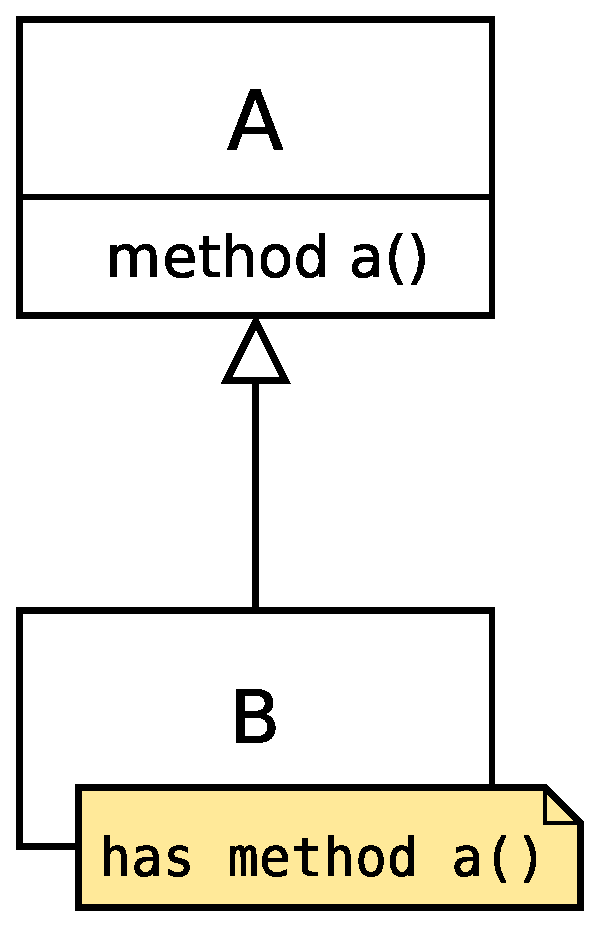
\includegraphics[scale = 0.27]{pictures/inheritance}
 \caption{Vererbung einer Methode.}
 \label{inheritance}
\end{figure}

Erbt eine Klasse von mehreren anderen Klassen, so nennt man das Mehrfachvererbung. Mehrfachvererbung war lange ein umstrittenes Thema in der objektorientierten Welt \cite{mi1}\cite{mi2}, denn sie kommt mit einer Herausforderung: Wie geht man damit um, wenn zwei gleichbenannte Methoden (oder Felder) geerbt werden? Eine sehr bekannte Ausprägung dieses Problems nennt sich das Diamond-Problem \cite{dp}. Es erhält seinen Namen von der Tatsache, dass die Vererbungshierarchie die Form einer Raute (englisch \emph{rhombus} oder \emph{diamond}) hat (Abb. \ref{diamond}):
Eine Klasse \texttt{D} erbt von zwei anderen Klassen \texttt{B} und \texttt{C}, die eine gemeinsame Superklasse \texttt{A} haben. Diese Superklasse hat ein Element (hier die Methode \texttt{a()}), das an beide Subklassen \texttt{B} und \texttt{C} vererbt wird und damit schlussendlich zweimal an \texttt{D}. Das Diamond-Problem ist nun die Fragestellung, wie die Klasse \texttt{D} damit umgeht.

\begin{figure}[h]
\centering
 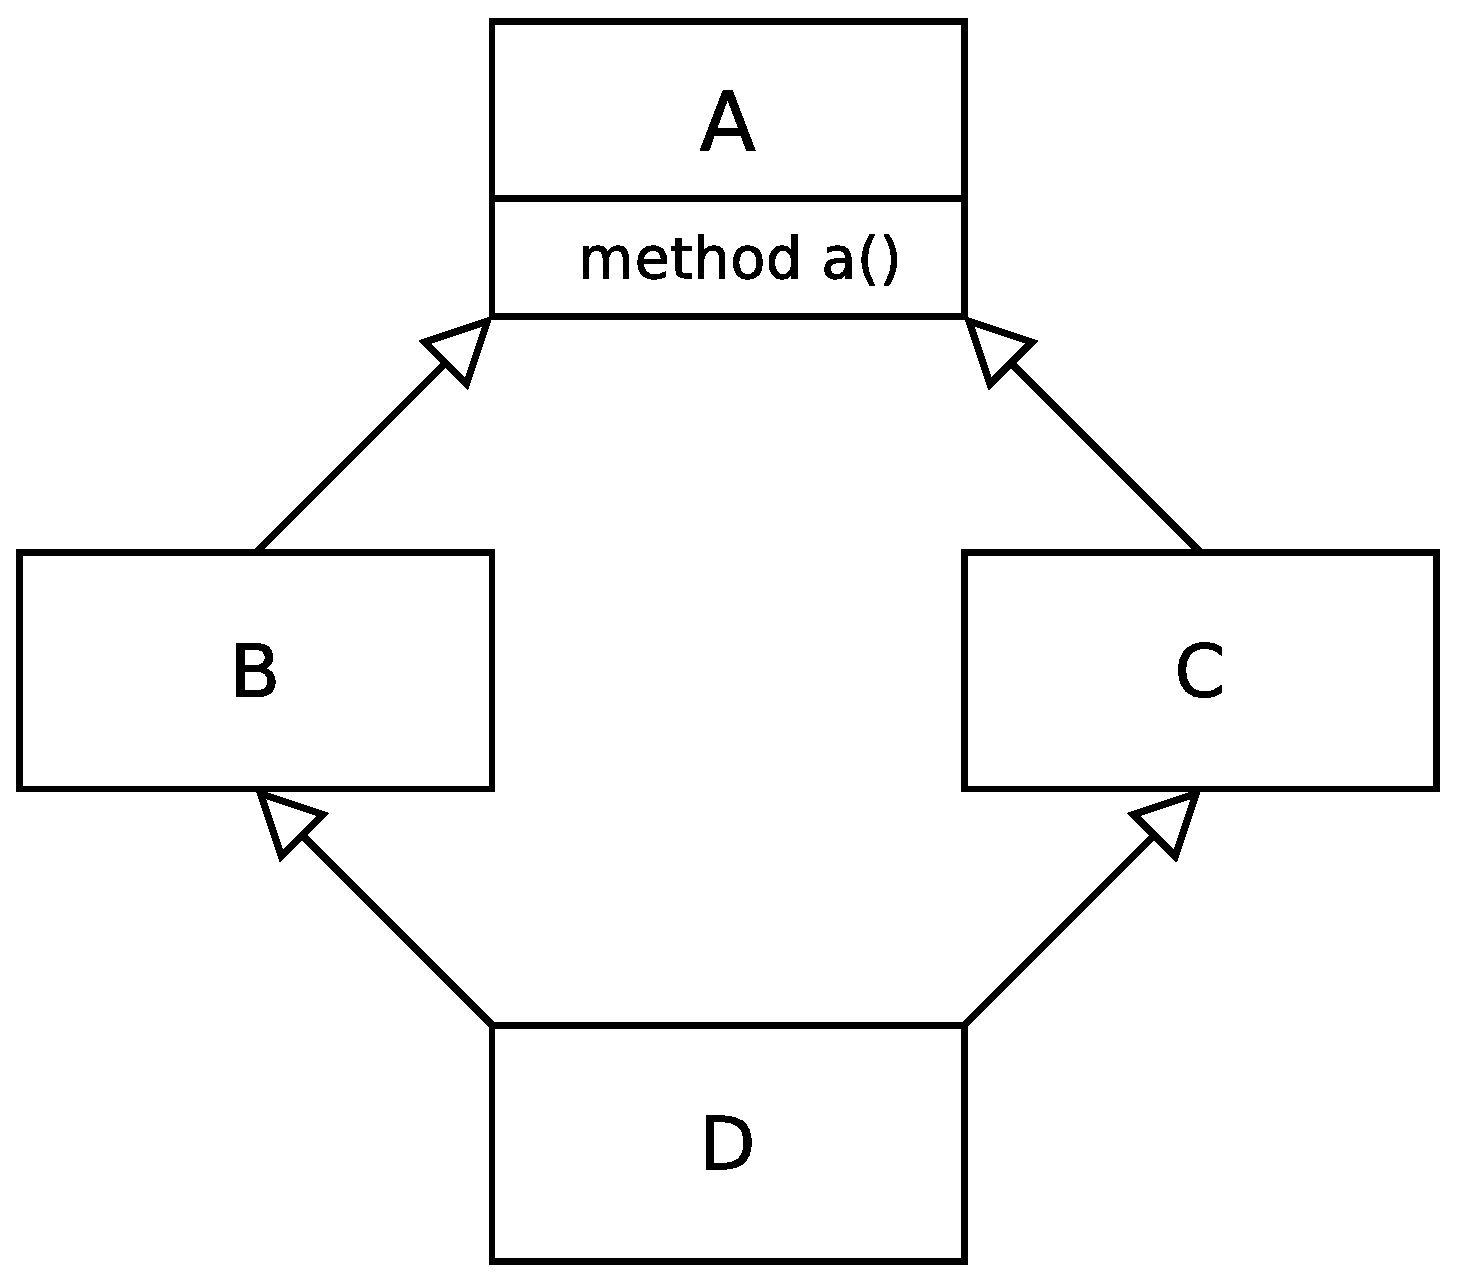
\includegraphics[scale = 0.27]{pictures/diamond}
 \caption{Das Diamond-Problem.}
 \label{diamond}
\end{figure}

Dafür haben sich im Laufe der Zeit in verschiedene Programmiersprachen (im folgenden: Sprachen) verschiedene Herangehensweisen entwickelt \cite{wikipedia}, die sich grob in sieben Strategien unterteilen lassen:

\begin{enumerate}
 \item Mehrfachvererbung wird nicht unterstützt. Als Alternative werden teils Mixins oder Traits genutzt. Beispiel: Java bis Version 7.
 \item Es ist nicht erlaubt, mehrdeutige Eigenschaften zu verwenden. Wenn in der Klasse \texttt{D} die Methode \texttt{a()} aufgerufen wird, so führt das zu einem Fehler. Beispiel: Go, Java 8.
 \item Zu vererbende Eigenschaften werden per Hand gewählt. Die Klasse \texttt{D} kann sich also entscheiden, entweder \texttt{B.a()} zu erben oder \texttt{C.a()}. Beispiel: Eiffel.
 \item Gleichbenannte Eigenschaften werden umbenannt. \texttt{D} würde zwei Methoden \texttt{ba()} und \texttt{ca()} erben. Beispiel: Eiffel, Logtalk.
 \item Man kann qualifiziert auf die Eigenschaften zugreifen. In \texttt{D} kann man dann mit \texttt{B.a()} oder \texttt{C.a()} die Methode aufrufen. Beispiel: C++, OCaml.
 \item Eigenschaften werden nach Präzedenz geerbt. Die Superklassen werden in eine bestimmte Reihenfolge (Präzedenzliste) gebracht und bei gleichbenannten Eigenschaften wird immer nur dasjenige geerbt, das in der Präzedenzliste zuerst kommt. Wenn wir beispielsweise die Klassen in die Reihenfolge \texttt{D,B,C,A} bringen, so würde die Eigenschaft je nach Implementierung entweder von \texttt{B} oder direkt von \texttt{A} geerbt, jedoch nur einmal. Beispiel: Common Lisp, Perl, Python.
 \item Kombination aller gleichbenannten Eigenschaften. Der Programmierer kann angeben, wie die geerbten Eigenschaften kombiniert werden sollen. Das funktioniert gegebenenfalls sogar für indirekte Superklassen. Haben \texttt{A} und \texttt{B} eine gemeinsame Eigenschaft, dann gehen beide in die Kombination mit ein. Beispiel: Common Lisp, Eiffel.
\end{enumerate}

% Für einen möglichst einfachen Einstieg in die Lehre von Mehrfachvererbung bietet sich Kategorie 6 am meisten an: Die Konfliktlösung passiert automatisch. Es reicht, eine Vererbungshierarchie anzugeben und den Rest übernimmt die Sprache. 

Racket nutzt die erste Strategie. Mehrfachvererbung wird nicht unterstützt.

Das Common Lisp Object System (CLOS) \cite{keene} vereint die Ansätze 6 und 7: Wird nichts anderes angegeben, so wird die Eigenschaft der Klasse mit der höchsten Präzedenz vererbt; der Programmierer hat jedoch für Methoden alternativ auch die Möglichkeit, eine Kombinationsart anzugeben. Diese Art der Mehrfachvererbung bietet auch einen einfachen Einstieg für die Lehre. Die Konfliktlösung ist automatisiert. Es reicht, eine Vererbungshierarchie anzugeben und den Rest übernimmt die Sprache. Gleichzeitig erhält der Programmierer durch Angabe einer Kombinationsart auch selbst die Möglichkeit der Kontrolle.

Die Funktionsweise von CLOS ist sehr ausführlich in dem Buch ``Object-oriented programming in Common Lisp. A programmer's guide to CLOS'' von Sonya E. Keene \cite{keene} dokumentiert. Einen Blick auf die Implementierung werfen Gregor Kiczales, Jim Des Rivieres und Daniel Gureasko Bobrow mit dem Werk ``The art of the metaobject protocol'' (AMOP) \cite{amop}. Sie zeigen, wie eine objektorientierte Sprache auf Basis von Lisp, Makros und Metaobjekten implementiert werden kann. 

Das Hinzufügen von Mehrfachvererbung zu einer bestehenden objektorientierten Sprache ist jedoch bisher wenig dokumentiert. 

\section{Motivation} 
An der Universität Hamburg gliedert sich die Lehre zur Softwareentwicklung in zwei Abschnitte. Im ersten Abschnitt werden in den Veranstaltungen ``Softwareentwicklung I'' und ``Softwareentwicklung II'' die Grundlagen für das Programmierverständnis gelegt. Die Studierenden erhalten einen  Einblick in imperative und objektorientierte Programmierung in Java nach dem Objects-First-Ansatz \cite{objectsfirst}.

Anschließend bieten die optionalen Module ``Softwareentwicklung III: Funktionale Programmierung'' sowie ``Softwareentwicklung III: Logikprogrammierung'' zusätzlich die Möglichkeit, zwei weitere  Programmierparadigmen kennenzulernen: funktionale Programmierung am Beispiel von Racket und logikbasierte Programmierung am Beispiel von Prolog.

Racket ist ein Dialekt der funktionalen Sprache Lisp. Genau wie Lisp hat Racket einen funktionalen Kern und ist gleichzeitig eine Mul\-ti\-pur\-pose-Spra\-che. Racket erlaubt es, neben dem funktionalen Stil auch imperative, obkjektorientierte und sogar logikbasierte Programme zu schreiben. Im Rahmen der Lehrveranstaltung werden daher auch diese Möglichkeiten aufgezeigt. 

Racket bietet zwei Arten, objektorientiert zu programmieren: ein integriertes Objektsystem, das sehr ähnlich zu Java ist, und eine Implementierung des Common Lisp Object Systems (CLOS), das eine eher funktionale Sicht auf die Objektorientierung hat. 

Da die Studierenden bereits aus ``Softwareentwicklung I'' und ``Softwareentwicklung II'' mit Java vertraut sind, bietet das Objektsystem von Racket kaum neue Lehrinhalte. Aus diesem Grund wird bisher CLOS, das in dem Racketdialekt Swindle implementiert ist, als Lehrinhalt behandelt. 

\section{Problemstellung} \vspace{-0.4cm}
Für die Implementation von CLOS wird ein so genanntes Metaobjektprotokoll verwendet, in dem Informationen über Klassen und Objekte durch interne Objekte verwaltet werden. In dieser Arbeit soll untersucht werden, ob das Metaobjektprotokoll auch genutzt werden kann, um Verhalten von CLOS zu dem bestehenden Objektsystem von Racket hinzuzufügen. Falls dies möglich ist, soll eine Spracherweiterung von Racket entwickelt werden. 

Die Spracherweiterung kann zukünftig im Rahmen der Lehre des Moduls ``Softwareentwicklung III'' genutzt werden, um Mehrfachvererbung direkt anhand des Objektsystems von Racket zu behandeln. Der Fokus liegt auf lehrrelaventen Konzepten: 
\begin{itemize}
 \vspace{0cm}
 \item Mehrfachvererbung\vspace{-0.5cm}
 \item Klassenpräzedenz\vspace{-0.5cm}
 \item Methodenkombination\vspace{-0.5cm}
 \item Ergänzungsmethoden
\end{itemize}

% Es ist bisher nicht möglich, diese Paradigmen in vollem Umfang im Objektsystem von Racket zu verwenden. Beide Systeme verwenden außerdem unterschiedliche Objekte, die nicht ohne weiteres miteinander kommunizieren oder ineinander umgewandelt werden können.
% 
% Im Rahmen dieser Arbeit soll eine Racket-Erweiterung entstehen, die Mehrfachvererbung auch im Objektsystem von Racket möglich ermöglicht. Als Anleitung soll die bereits existierende Umsetzung in CLOS dienen. 


\section{Vorgehen}
Um über Mehrfachvererbung in Racket und CLOS reden zu können, werden im Kapitel \textbf{Objektsysteme in Racket} die Sprache Racket und die existierenden Objektsysteme beschrieben. Das Kapitel soll ein Gefühl dafür geben, wie die beiden Systeme zu benutzen sind und Gemeinsamkeiten, Unterschiede und Grenzen aufzeigen.

Anschließend wird im Kapitel \textbf{Entwurf} ein Vorschlag gemacht, auf welche Weise Racket um Mehrfachvererbung erweitert werden kann. 

Im Kapitel \textbf{Analyse der Implementierungsdetails von CLOS} wird anhand der Implementierung von CLOS ergründet, wie das Metaobjektprotokoll genutzt werden kann, um ein bestehendes Objektsystem um die Möglichkeit von Mehrfachvererbung zu erweitern. Es werden relevante Implementierungsdetails von CLOS beschrieben und ihre Anwendbarkeit auf das Objektsystem von Racket evaluiert.

Das Kapitel \textbf{Umsetzung} beschreibt den in dieser Arbeit entstandenen Prototypen und beleuchtet Abweichungen zu CLOS sowie Probleme, die bei der Umsetzung auftraten und wie sie gelöst wurden.

In der \textbf{Auswertung} wird der entstandene Prototyp getestet. Es werden Einschränkungen, die gemacht werden mussten, beleuchtet und ein Fazit über die Eignung des Metaobjektprotokolls zur Erweiterung eines Objektsystems gezogen.

Zum Abschluss werden in \textbf{Zusammenfassung und Ausblick} noch einmal die Ergebnisse zusammengefasst und Möglichkeiten der Erweiterung diskutiert.

\section{Beiliegende CD}
Auf der beiliegenden CD befindet sich eine digitale Version dieser Arbeit sowie der entstandene Prototyp und eine Zusammenstellung der behandelten Beispiele als Racketdateien.

 % TODO ausformulieren
\chapter{Objektsysteme in Racket}
Racket ist ein Dialekt von Lisp, der auf Scheme basiert. Es ist jedoch keine rein funktionale Sprache, sondern unterstützt verschiedene Lisp-Dialekte und  Programmierparadigmen. 
%Damit gibt Racket Programmierern und Forschern die Werkzeuge, die sie benötigen, um neue Sprachen zu erkunden und zu entwickeln\cite{racketguide-dialects} und wird beispielsweise auch an der Universität Hamburg in der Forschung genutzt.

Racket wird in der Softwareentwicklungslehre genutzt, da es im Gegensatz zu Common Lisp sehr einsteigerfreundlich ist. Die Veranstaltungsteilnehmer lernen zum ersten Mal eine funktionale Sprache kennen und sollen einen möglichst einfachen Einstieg erhalten. Hierzu bietet Racket eine übersichtliche Syntax und eine plattformunabhängige Entwicklungsumgebung, die vergleichbare Fehlermeldungen liefert.

In Common Lisp wird die Syntax schnell sehr komplex und ist zudem abhängig von der Implementierung (teilweise sogar mit kostenpflichtigem Interpreter). Common Lisp hat zwei verschiedene Paketsysteme mit tausenden von Paketen, was ein schnelles Zurechtfinden in der Sprache nicht unbedingt begünstigt. Es gibt keine dedizierte grafische Oberfläche, da Common Lisp für die Integration in Emacs, Vim etc. ausgelegt ist. Das würde bedeuten, dass Veranstaltungsteilnehmer sich erst einmal mit der Integration der Sprache in den Editor ihrer Wahl beschäftigen müssten, bevor sie überhaupt eine Zeile Code schreiben können. Nicht alle Interpreter von Common Lisp werden auch für alle Betriebssysteme gewartet, wie zum Beispiel SBCL, der zwar frei und gut ist, aber unter Windows nur gelegentlich gepflegt wird. Das macht es extrem schwer die Ursache von Fehlern zu erkennen, da immer auch das Betriebssystem bedacht werden muss. Zudem ist eine systemübergreifende grafische Ausgabe ohne weitere Pakete nicht vorgesehen. Das erschwert das Stellen von Aufgaben, bei denen das Ergebnis visualisiert werden kann oder muss, da die grafische Ausgabe vom Interpreter abhängig ist und die Teilnehmer zudem erst einmal die entprechenden Pakete installieren müssten. 

Um Common Lisp zu lernen, wurde daher Scheme entwickelt. Analog zu BlueJ, einer Entwicklungsumgebung für das Lernen von objektorientierter Programmierung in Java, war DrScheme das Einsteigertool zu Common Lisp. Im Jahr 2010 wurde Scheme umbenannt zu Racket. Racket bildet einen guten Kompromiss für die Lehre, da es einen einfachen Einstieg in die Welt von Common Lisp bietet.
%----------------------

Die Syntax von Racket ist sehr ähnlich zu Common Lisp. Ausdrücke werden geklammert, Kommentare mit einem Semikolon eingeleitet. Einige Standardfunktionen haben leicht abgewandelte Namen. So werden in Racket beispielsweise sowohl Funktionen als auch Variablen mit dem Schlüsselwort \texttt{define} definiert, anstelle von \texttt{defun}, \texttt{defvar} und \texttt{defparameter} in Common Lisp. Prädikate enden auf \texttt{?} (zum Beispiel \texttt{equal?}) und Methoden, die Variablen oder Objekte verändern auf \texttt{!} (zum Beispiel \texttt{set!}). Einer der größeren Unterschiede liegt in der Art, wie Makros definiert werden; darauf wird im Kapitel \ref{makros} noch näher eingegangen.

Racket unterstützt auch objektorientierte Programmierung auf zwei verschiedene Arten. Zunächst gibt das Racket-Objektsystem. Racket-Klassen sind sehr ähnlich zu Klassen in Java, C\# oder den meisten objektorientierten Programmiersprachen. Ein Programm kann Klassen definieren, instanziieren, mit den erzeugten Objekten interagieren und Klassen erweitern. Besonders ist, dass Klassen auch wie Funktionswerte behandelt werden können. Es ist möglich, eine Klasse zur Laufzeit zu erweitern, eine Klasse an eine Funktion zu geben oder in einer Datenstruktur zu speichern und anschließend abzufragen \cite{neu-edu}. 

Zusätzlich gibt es den Racket-Dialekt Swindle, in dem das Common Lisp Object System (CLOS) implementiert ist. Im Gegensatz zum eingebauten Objektsystem von Racket bietet CLOS Funktionalitäten wie Mehrfachvererbung, Methodenkombination oder Ergänzungsmethoden. Durch die Implementation als Metaobject-Protocol bietet es dem Programmierer zudem viel Freiheit bei der Erweiterung und Veränderung der Repräsentation von Klassen und Objekten.
Um ein Gefühl für die beiden Objektsysteme zu bekommen, soll zunächst betrachtet werden, wie sie benutzt werden können. %Andschließend wird ein Blick auf die Implementation beider Ansätze geworfen. Die Autoren des Buches ``The Art of the Metaobject Protocol''\cite{amop} vergleichen das Vorgehen sehr treffend mit eine Theateraufführung: Auf der Bühne (onstage) findet das Theaterstück statt - das Programm, oder etwas allgemeiner, das, was der Programmierer von der Sprache sieht. Hinter der Bühne (backstage) befindet sich die darunterliegende Implementation, die die entprechenden Makros definiert und mit für den Programmierer nicht sichtbaren Objekten und Funktionen arbeitet. Wir wollen beide Ansätze erst ``onstage'' betrachten bevor wir einen Blick hinter die Kulissen werfen.

Der Fokus dieser Arbeit liegt auf der Implementation von Mehrfachvererbung im Objektsystem von Racket. Natürlich bieten sowohl das Objektsystem von Racket als auch CLOS neben Vererbung auch noch viele weitere nützliche Funktionen und Eigenschaften; diese sind jedoch nicht zielführend für diese Arbeit und es würde eine eigene Ausarbeitung benötigen, sie alle aufzulisten. Im Folgenden wird daher nur auf diejenigen Bestandteile beider Ansätze eingegangen, die direkt oder indirekt mit Mehrfachvererbung zu tun haben. 

Die Installation von Racket beinhaltet eine integrierte Enwicklungsumgebung namens DrRacket. Für das Syntaxhighlighting der Quelltextbeispiele in dieser Arbeit wurde das Standard-Farbschema von DrRacket verwendet. Anfragen an die Interaktionskonsole wurden mit \texttt{>} markiert und das Ergebnis in der Zeile darunter aufgeführt. 

\section{Ein Beispiel für Mehrfachvererbung} 

Wir wollen beide Ansätze in Hinblick auf Syntax, Benutzung und Vererbung miteinander vergleichen. Dazu soll in beiden die folgende Vererbungshierarchie implementiert werden:

\begin{figure}[h]
 \centering
 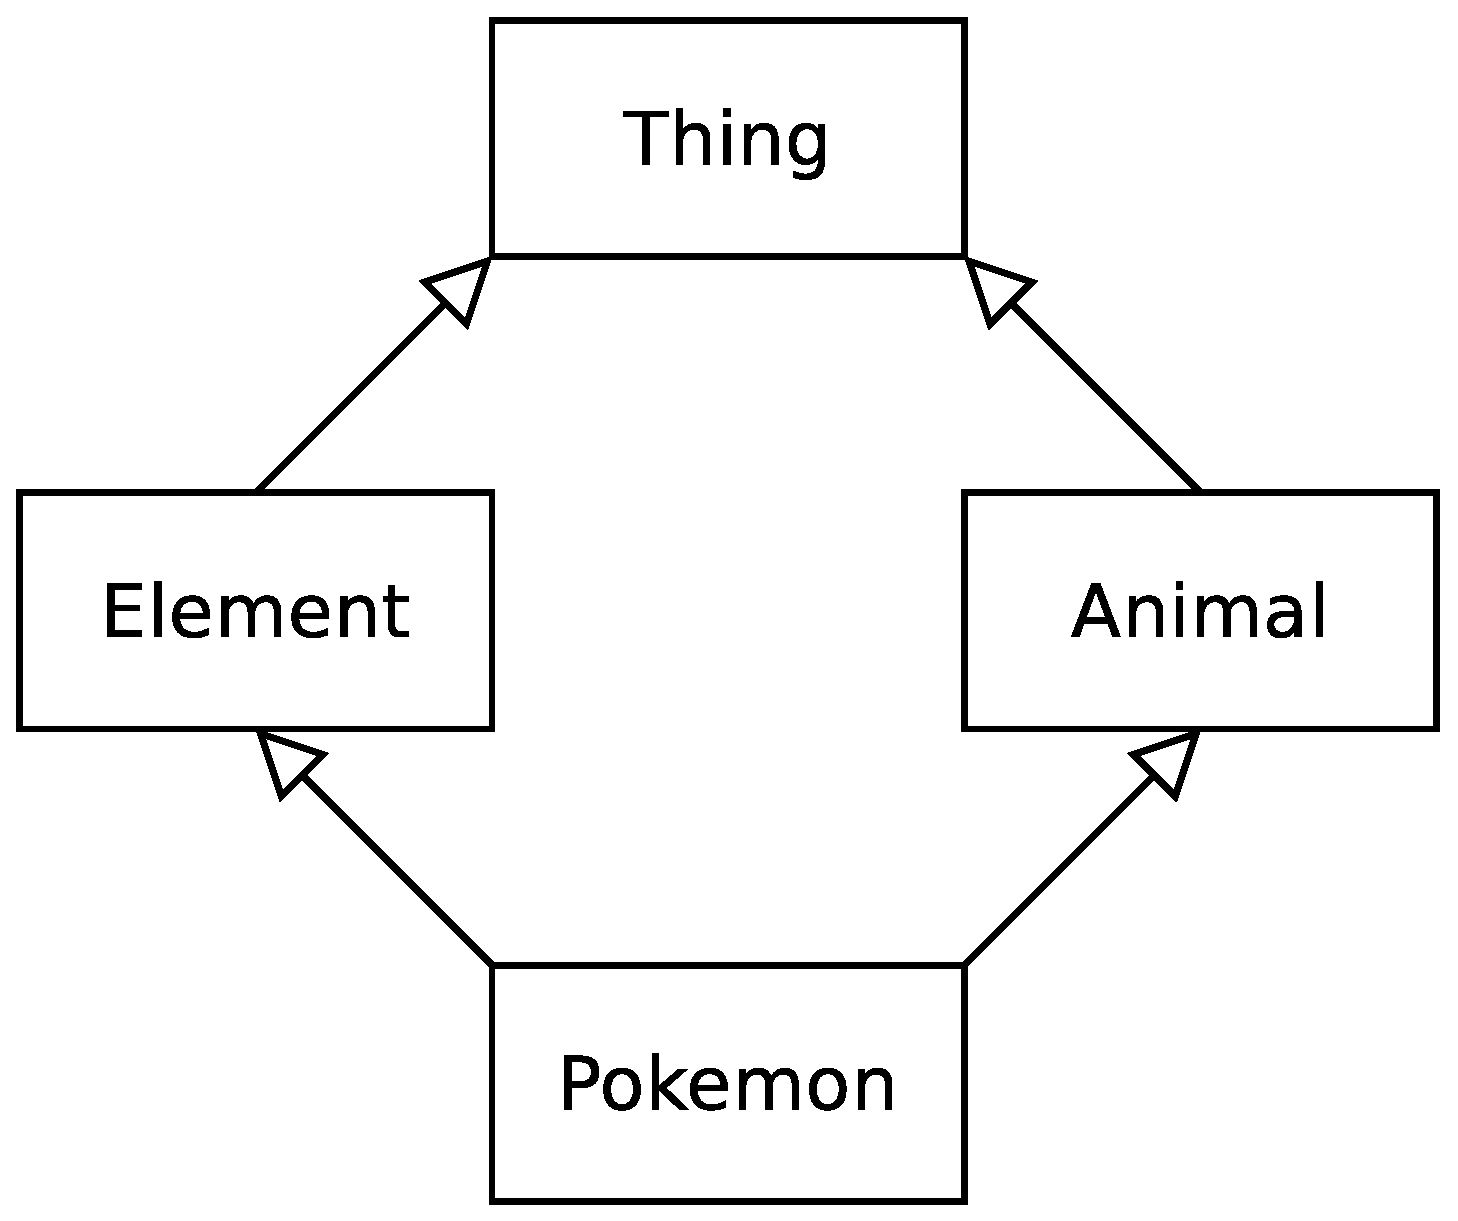
\includegraphics[scale=0.3]{pictures/pokemon}
 \caption{Vererbungshierarchie für die Klasse Pokemon.}
 \label{pokemon}
\end{figure}

Zunächst können wir mit der Klasse Thing sehen, wie eine einfache Klasse definiert wird. Anhand von Thing und den Klassen Element und Animal betrachten wir, wie Felder und Methoden definiert werden können und wie diese vererbt werden.

Schließlich vervollständigen wir die Hierarchie so, dass mit möglichst wenig Klassen möglichst viele Sonderfälle und Probleme abgedeckt werden können. Hierfür eignet sich das Diamant-Problem sehr gut: Eine Klasse, die von zwei Klassen erbt, die wiederum eine gemeinsame Superklasse haben. Element und Animal erben bereits von Thing. Wir nutzen den Umstand also aus und definieren eine Klasse Pokemon, die von beiden erbt.

In jedem Schritt wollen wir betrachten, was passiert, wenn man Methoden redefiniert, wie disjunkte Mengen von Slots und Methoden vererbt werden, wie mit gleichbenannten Merkmalen umgegangen wird und wie man als Programmierer die Vererbung bei gleichbenannten Merkmalen beeinflussen kann.

Zusätzlich wollen wir noch betrachten, welche Möglichkeiten es gibt, Methoden einer Superklasse in einer Subklasse zu ergänzen und ob diese kompatibel mit Mehrfachvererbung sind (und wenn nicht, warum).
\section{Das Objektsystem von Racket: Onstage}
Als Grundlage für dieses Kapitel dient die Racket-Dokumentation \cite{racketguide-classes} und -Referenz \cite{racketref-classes} für Klassen und Objekte.

Racket ist eine Multipurpose-Sprache und erlaubt die Auswahl der Syntax auf Sprachebene. Eine einzelne Codezeile bestimmt die Sprache eines Moduls, also beispielsweise, ob die Funktionen vorgezogen ausgewertet werden (\texttt{\#lang racket}) oder verzögert (\texttt{\#lang lazy}). Da das Objektsystem in die Sprache Racket integiert ist, kann man es direkt in jedem Racket-Modul verwenden.

% \begin{lstlisting}
%  #lang racket
% \end{lstlisting}

Die wichtigsten Werkzeuge, die man als Programmierer in einer objektorientierten Sprache benötigt, sind das Definieren von Klassen, Feldern und Funktionen, sowie das Erzeugen von Objekten. Auf diese soll deshalb im Folgenden kurz eingegangen werden, bevor wir dazu kommen, welche Möglichkeiten es in Bezug auf Mehrfachvererbung im Objektsystem von Racket bereits gibt.

Alle Code-Beispiele sind auch noch einmal zusammenhängend in Anhang \ref{or-example} aufgeführt. 

\subsection{Einfache Klassen}

Eine Klasse wird in Racket durch das Schlüsselwort \texttt{class} definiert. Bei der Definition einer Klasse muss die Superklasse angegeben werden. Falls die Klasse keine (anderen) Superklassen hat, wird \texttt{object\%} angegeben, die eingebaute Wurzelklasse. Per Konvention sollen Klassennamen in Racket auf \% ended, bei den folgenden Beispielen wird jedoch darauf verzichtet, um sie später leichter mit CLOS vergleichen zu können. Nach der Superklasse können noch beliebige Klassenoptionen, Felder oder Methoden definiert werden. An einer beliebigen Stelle im Rumpf der Klasse muss jedoch mit \texttt{super-new} der Konstruktor der Oberklasse aufgerufen werden. Eine minimale Klassendefinition sieht damit folgendermaßen aus:

\begin{lstlisting}
(class object% (super-new))
\end{lstlisting}

Als Rückgabewert erhält man ein Klassenobjekt und kann dieses für den späteren Zugriff in einer Variablen speichern. Die Variable wurde hier Thing genannt.

\begin{lstlisting}
(define Thing (class object% (super-new)))
\end{lstlisting}

Objekte von Klassen lassen sich mit dem Schlüsselwort \texttt{new} erzeugen:

\begin{lstlisting}
(new Thing)
\end{lstlisting}

Felder lassen sich mit \texttt{init-field} oder \texttt{field} deklarieren, je nachdem, ob es möglich sein soll sie bei der Objekterzeugung zu initialisieren oder nicht. Auf die Felder kann man dann mit \texttt{get-field} beziehungsweise \texttt{set-field!} zugreifen. 

Für Methoden gibt es, je nach Art und Sichtbarkeit, unter anderem die Schlüsselwörter \texttt{define/public}, \texttt{define/private} und \texttt{define/override}. Die so definierten Methoden lassen sich anschließend mittels \texttt{send} aufrufen. Zum Beispiel sieht eine Klasse namens Element, bestehend aus einem Feld für das Attribut und einer sondierenden Methode, die von Thing erbt, folgendermaßen aus:

\begin{lstlisting}
(define Element (class Thing (super-new)
                  (init-field [attr 'water])
                  (define/public (hot?) (equal? attr 'fire))))
\end{lstlisting}

Attribute, die keinen Defaultwert haben, müssen bei der Initialisierung angegeben werden. Da das Attribut der Element-Klasse, hier \texttt{attr} genannt, \texttt{{\textquotesingle}water} als Defaultwert hat, ist eine Angabe bei der Objekterzeugung optional. Mit den Methoden \texttt{get-attr} und \texttt{set-attr} können wir darauf zugreifen:

% > elem
% \end{lstlisting} 
% {\routput (object:Element ...)}

\begin{lstlisting}
(define elem (new Element))

> (get-field attr elem)
\end{lstlisting} 
{\rsymbol{water}}
\begin{lstlisting}
> (send elem hot?)
\end{lstlisting} 
{\routput{\#f}}

\begin{lstlisting}
> (set-field! elem attr 'fire)
> (send elem hot?)
\end{lstlisting} 
{\routput{\#t}}
% 
% \begin{lstlisting}
% (define elem2 (new Element [attr 'fire]))
% 
% > (send elem2 get-attr)
% \end{lstlisting} 
% {\rsymbol{fire}}

Wir können uns auch eine Klasse Animal definieren, die von Thing erbt (auch wenn es nicht viel zu vererben gibt):

\begin{lstlisting}
(define Animal (class Thing (super-new)
                 (init-field [gender 'male]
                             [size 'small])))
\end{lstlisting} 

Und eine Klasse Pet, die wiederum von Animal erbt:

\begin{lstlisting}
(define Pet (class Animal (super-new)
              (init-field [name 'unknown])))
\end{lstlisting} 

Objekte der Klasse Pet besitzen dann alle drei Attribute:

\begin{lstlisting}
(define harry (new Pet [name 'harry] [size 'normal]))

> (get-field name harry)
\end{lstlisting} 
{\rsymbol harry}

\begin{lstlisting}
> (get-field gender harry)
\end{lstlisting} 
{\rsymbol male}

\begin{lstlisting}
> (get-field size harry)
\end{lstlisting} 
{\rsymbol normal}

% TODO The make-object procedure creates a new object with by-position initialization arguments, the new form creates a new object with by-name initialization arguments, and the instantiate form creates a new object with both by-position and by-name initialization arguments.

\subsection{Mehrfachvererbung in Racket}
Zuvor wurde behauptet, mit Racket könne man keine Mehrfachvererbung modellieren. Tatsächlich gibt es zwei Arten von Klassen in Racket, deren Verhalten auf den ersten Blick wie Mehrfachvererbung aussieht: Mixins und Traits. Es werden deshalb beide kurz vorgestellt, um aufzuzeigen, welche Probleme und Grenzen sie haben.

Dafür verwenden wir unsere vorher definierten Klassen Element und Animal. Beide haben unterschiedliche Felder und Methoden. Wir wollen versuchen, die Felder und Methoden aus beiden in einer neuen Klasse namens Pokemon zu vereinigen (Abbildung \ref{hirarchy}). Das ginge natürlich ganz simpel, indem eine der beiden Klassen in Pokemon umbenannt wird und von der anderen erbt, deshalb wollen wir außerdem fordern, dass beide Klassen auch einzeln verwendet können. 

\begin{figure}[h]
 \centering
 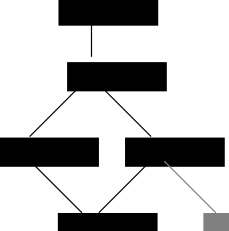
\includegraphics[width=0.35\textwidth]{pictures/hirarchy}
 \caption{Vererbungshierarchie für die Klasse Pokemon.}
 \label{hirarchy}
\end{figure}


\subsubsection{Mixins}
Die Auswertung eines \texttt{class}-Aufrufs gibt uns ein Klassenobjekt zurück. Es möglich, dieses als Parameter an Funktionen oder andere Klassen zu übergeben oder auch als Rückgabewert eines Funktionsaufruf zu definieren. Wir könnten uns beispielsweise eine Methode \texttt{generate-subclass} definieren, die eine Klasse als Parameter erhält und eine Subklasse von dieser erzeugt. Dafür muss sie den Parameter nur als Superklasse in einer Klassendefinition verwenden:

\begin{lstlisting}
(define (generate-subclass superclass)
  (class superclass (super-new)))
\end{lstlisting} 

Das ist noch keine sonderlich spannende Subklasse, da sie sich genauso verhält wie die angegebene Superklasse.
% aber wir können uns von ihrer Funktionalität überzeugen. Nehmen wir beispielsweise eine Subklasse der Klasse Element:
% 
% \begin{lstlisting}
% > (generate-subclass Element) 
% \end{lstlisting}
% {\routput \#<class:...>}
% 
% Dann erhalten wir das gleiche Verhalten wie für Objekte der Klasse Element:
% 
% \begin{lstlisting}
% > (new (generate-subclass Element))
% \end{lstlisting}
% {\routput (object:...)}
% 
% \begin{lstlisting}
% > (send (new (generate-subclass Element)) get-attr)
% \end{lstlisting}
% {\rsymbol water}
% 
Nun könnte man in der in \texttt{generate-} \texttt{subclass} definierten Klasse natürlich auch noch weitere Felder und Methoden hinzufügen. Die Klasse fügt dann Verhalten zu einer bestehenden, aber noch unbekannten Klasse hinzu. Erst beim Methodenaufruf wird der Platzhalter mit einer tatsächlichen Superklasse gefüllt. Eine solche Klasse wird in Racket Mixin genannt und als Platzhalter für die Superklasse wird per Konvention \texttt{\%} genommen:

\begin{lstlisting}
(define (a-mixin %)
  (class % (super-new)
    ; neues Verhalten
    ))
\end{lstlisting}

Falls wir das Verhalten beider Klassen Element und Animal vereinen wollen, so könnten wir eine von ihnen, oder beide, als Mixin definieren. Beide Klassen als Mixin zu definieren kommt am nächsten an unsere Idee von Mehrfachvererbung:

\begin{lstlisting}
(define (Element-mixin %)
  (class % (super-new)
    (init-field [attr 'water])))

(define (Animal-mixin %)
  (class % (super-new)
    (init-field [gender 'male]
                [size 'small])))
\end{lstlisting}

Und aus diesen könnten wir uns dann alle drei Klassen Element, Animal und Pokemon erzeugen:
\begin{lstlisting}
(define Element (Element-mixin Thing))

(define Animal (Animal-mixin Thing))
 
(define Pokemon (Element-mixin (Animal-mixin Thing)))
\end{lstlisting}

Es wird Thing als Superklasse verwendet, da sie zuvor als leere Klasse definiert wurde. Genausogut hätten wir natürlich \texttt{object\%} benutzen können. Es fällt auf, dass die zwei Mixins nicht gleichwertig sind; wir müssen uns entscheiden, welches von beiden wir zuerst anwenden. Genau genommen passiert hier auch keine Mehrfachvererbung, sondern zweifache Einfachvererbung -- mit dem Vorteil jedoch, dass wir die zwei Klassen auch unabhängig voneinander verwenden können. Die Hierarchie sieht also wie folgt aus:

\texttt{Pokemon $\rightarrow$ Element $\rightarrow$ Animal $\rightarrow$ Thing $\rightarrow$ object\%}

Element und Animal verhalten sich genauso wie zuvor:

\begin{lstlisting}
> (get-field attr (new Element))
\end{lstlisting} 
{\rsymbol{fire}}

\begin{lstlisting}
> (get-field size (new Animal [size 'huge] [gender 'female]))
\end{lstlisting} 
{\rsymbol{huge}}

Zusätzlich können wir uns nun auch ein Pokemon definieren, das alle drei Eigenschaften aufweist:
\begin{lstlisting}
(define p (new Pokemon [size 'large]
                       [gender 'female]
                       [attr 'fire]))
 
> (get-field size p)
\end{lstlisting}
{\rsymbol{large}}
\begin{lstlisting}
> (get-field gender p)
\end{lstlisting}
{\rsymbol{female}}
\begin{lstlisting}
> (get-field attr p)
\end{lstlisting}
{\rsymbol{fire}}

Falls es also nicht stört, dass technisch eigentlich keine Mehrfachvererbung geschieht, so scheinen sich Mixins zunächst gut zur Modellierung zu eignen. Es muss lediglich für jede Klasse, die für Mehrfachvererbung in Frage kommt, eine Mixin-Klasse definiert werden. Einen Umstand haben wir jedoch bisher außen vor gelassen: gleichbenannte Felder und Methoden. Element und Animal besitzen bisher eine disjunkte Menge von Feldern und Methoden. 

Das soll sich nun ändern. Nehmen wir an, es gibt eine Funktion \texttt{attack}, die sowohl Element als auch Animal haben. Ein Angriff des Elements Feuer soll einfach Feuer sein, bei Tieren sagen wir, der Angriff ist proportional zur Größe und auf Pokemon trifft beides zu. Der Einfachheit halber gibt die Funktion für Element und Animal also einfach die Werte der Felder \texttt{attr} und \texttt{size} zurück:

\begin{lstlisting}
(define (Element-mixin %) ...
    (define/public (attack) attr))
 
(define (Animal-mixin %) ...
    (define/public (attack) size))
\end{lstlisting}

Nun schlägt jedoch die Definition der Klasse Pokemon fehl:

\begin{lstlisting}
> (define Pokemon (Element-mixin (Animal-mixin Thing)))
\end{lstlisting}
{\rerror $\bigotimes$ class*: superclass already contains method\\
method name: attack}

Racket erlaubt es nicht, dass zwei Methoden in einer Klasse den gleichen Namen haben. Wir dürfen geerbte Methoden aus Superklassen nicht neu deklarieren. Falls wir vorhaben, sie zu überschreiben, so müssen wir \texttt{define/override} verwenden:

\begin{lstlisting}
(define (Element-mixin %) ...
    (define/override (attack) attr))
\end{lstlisting}

Das führt jedoch dazu, dass wir nun bei der Erstellung der Element-Klasse nicht mehr Thing als Superklasse angeben können, denn die Klasse Thing bietet keine Funktion \texttt{attack}, die überschrieben werden könnte. Wollen wir also weiterhin, dass es möglich ist, sich Objekte von der Klasse Element zu erzeugen, so müssen wir eine Klasse bereitstellen, die eine solche Methode anbietet, damit Element von ihr erben kann.

\begin{lstlisting}
(define Element 
  (Element-mixin (class object% (super-new)
                   (define/public (attack) null))))
\end{lstlisting}

Zudem ist der Angriff eines Pokemons nun ledligchlich der Wert des Feldes \texttt{attr}. 
% Für unser Pokemon \texttt{p} von oben ergibt das:
% \begin{lstlisting}
% > (send p attack)
% \end{lstlisting}
% {\rsymbol fire}
% 
Was wir eigentlich wollen, ist jedoch eine Kombination aus der Größe und dem Element. Das heißt, damit Pokemon das gewünschte Verhalten zeigt, müsste Element eine Kombination aus dem eigenen Wert und dem der Superklasse zurückgeben.

\begin{lstlisting}
(define (Element-mixin %) ...
    (define/override (attack) (list (super attack) attr)))
\end{lstlisting}

Abgesehen davon, dass es kein sehr guter Programmierstil ist, die Logik der Klasse Pokemon in eine andere Klasse auszulagern, hat es wiederum Einfluss auf Objekte der Klasse Element. Anstatt des Attributs erhält man nun eine etwas seltsam anmutende Liste:

\begin{lstlisting}
> (send (new Element) attack)
\end{lstlisting}
{\rsymbol (() water)}

Dafür zeigt Pokemon nun das gewünschte Verhalten.
\begin{lstlisting}
> (send p attack)
\end{lstlisting}
{\rsymbol (large fire)}

Es ist jedoch nicht mehr möglich, die Reihenfolge der Mixins zu vertauschen. Eine Definition von Pokemon als

\begin{lstlisting}
(define Pokemon (Animal-mixin (Element-mixin Thing)))
\end{lstlisting}

führt zu einem Fehler, aus dem gleichen Grund wie vorher bei Objekten der Klasse Element: da Element eine Superklasse erwartet, die eine Funktion \texttt{attack} anbietet. Da Thing nun die direkte Superklasse ist, ist das nicht mehr der Fall. Selbst wenn wir das beheben würden, würde die Erzeugung nun an Animal scheitern, da es die geerbte Methode aus Element nicht überschreibt, sondern versucht neu zu definieren. Wir müssten alle Schritte, die wir soeben zur erfolgreichen Vererbung von der Methode \texttt{attack} durchgeführt haben, für den umgekehrten Fall definieren. 

Wollen wir beide Vererbungs-Reihenfolgen erlauben, wird zudem die Funktion \texttt{attack} deutlich komplizierter, da nun anhand der Superklasse entschieden werden müsste, ob der Wert des Feldes direkt zurückgegeben werden kann oder eine Kombination mit dem Wert der Superklasse nötig ist.

Wir haben bisher nur zwei Superklassen betrachtet. Bei drei, vier oder gar 20 Superklassen, die vielleicht selbst wiederum von mehreren Superklassen erben, wird, falls eine sinnvolle Modellierung mit Mixins überhaupt noch möglich ist, der Code extrem unübersichtlich und schwer wartbar. Insbesondere für die Lehre von Mehrfachvererbung eignen sie sich demnach nicht.

\subsubsection{Traits}
Traits sind ähnlich zu Mixins. Sie kapseln eine Menge von Methoden, die zu einer Klasse hinzugefügt werden sollen. Traits erlauben jedoch Kontrolle darüber, welche Methoden wie geerbt werden. Es ist möglich bestimmte Methoden nicht zu erben, sie unter einem Alias zu erben oder mit Trait-Operatoren zu manipulieren und die Ergebnisse mehrerer Methoden zu kombinieren.

Sie lösen damit eines der fundamentalen Probleme von Mixins: Die Vererbung und Kombination gleichbenannter Methoden. Wenn es in zwei Traits, die kombiniert werden sollen, gleichbenannte Methoden gibt, so hat der Programmierer die Möglichkeit (und Pflicht), anzugeben, wie diese Kollision gelöst werden soll -- üblicherweise durch Ausschließen oder Umbenennen einer der Methoden in der Subklasse, oder durch Methodenkombination.

Die Definition von Traits ist syntaktisch fast identisch zu der Definition einer Klasse, es gibt nur zwei Unterschiede: Anstelle des Schlüssworts \texttt{class} wird \texttt{trait} benutzt und es müssen weder Superklasse noch Superkonstruktor-Aufruf angegeben werden. Traits unterstützen einen Großteil der Optionen, die auch \texttt{class} unterstützt, unter anderem aber keine \texttt{init-field}s. Prinzipiell können wir jedoch unsere Defintion für Element und Animal fast eins zu eins übernehmen. 

\begin{lstlisting}
(require racket/trait)

(define Element-trait
  (trait (field [attr 'water]) ; statt init-field
         (define/public (attack) attr)))

(define Animal-trait
  (trait (field [gender 'male] ; statt init-field
                [size 'small])
         (define/public (attack) size)))
\end{lstlisting}

Wenn wir ein Pokemon-Trait aus diesen beiden Traits definieren wollen, müssen wir den Konflikt der beiden \texttt{attack}-Methoden beheben. Das geht jedoch im Gegensatz zu Mixins direkt im Pokemon-Trait. Zur Manipulation der Vererbung gibt verschiedene Trait-Operationen, wie
\begin{itemize}
 \item \texttt{trait-exclude}, das eine Methode von einem Trait entfernt,
 \item \texttt{trait-alias}, welches die Kopie einer Methode unter anderem Namen zum Trait hinzufügt und
 \item \texttt{trait-sum}, welche die Methoden von zwei Traits kombiniert.
\end{itemize}

Das Vorgehen bei einem Konflikt lässt sich generalisieren. Zunächst wird dafür gesorgt, dass es keinen Namenskonflikt mehr gibt. Dafür wird aus den zwei Traits mit kollidierender Methode jeweils ein neuer Trait erstellt, in dem diese Methode einen neuen, eindeutigen Namen erhält. Dafür würden wir beispielweise zum Trait Element mit \texttt{trait-alias} einen Alias für die \texttt{attack}-Methode hinzufügen, den wir \texttt{element-attack} nennen. Der Trait hat anschließend \emph{zwei} Funktionen für den Angriff, \texttt{attack} und \texttt{element-attack}, die beide das gleiche tun. Anschließend können wir mit \texttt{trait-exclude} die ursprüngliche \texttt{attack}-Methode von der Vererbung ausschließen. Es wird also nur die Alias-Methode \texttt{element-attack} vererbt.

Dieser Schritt wird für jeden Konflikt durchgeführt. Sobald alle Methoden einen eindeutigen Namen haben, können sie dann mit \texttt{trait-sum} kombiniert werden.

\begin{lstlisting}
 (define Pokemon-trait
   (trait-sum   ; Kombiniere die folgenden Traits
    (trait-exclude (trait-alias Element-trait   ; Erstelle Alias fuer
                                attack          ; attack und entferne
                                element-attack) ; das Original
                   attack)
    (trait-exclude (trait-alias Animal-trait    ; Analog fuer Animal
                                attack         
                                animal-attack)
                   attack)
    (trait (inherit element-attack animal-attack) ; Kombiniere die zwei
           (define/public (attack)                ; attack-Methoden
             (list (animal-attack) (element-attack))))))
\end{lstlisting}

Wir erhalten einen neuen Trait. 

\begin{lstlisting}
> Pokemon-trait
\end{lstlisting}
{\routput \#<trait>}

Man kann Traits nicht direkt zu Klassen hinzufügen, aber man kann sie mit der Funktion \texttt{trait->mixin} in ein Mixin umwandeln und dieses dann zu einer Klasse hinzufügen:

\begin{lstlisting}
 (define Pokemon ((trait->mixin Pokemon-trait) Thing))
\end{lstlisting}

Da wir \texttt{field} statt \texttt{init-field} bei der Traitdefinition benutzt haben, ist es nun jedoch nicht mehr möglich, die Felder zu initialisieren. Man kann zwar im Rumpf der Klasse per Hand \texttt{init} aufrufen und damit eine Initialisierung erzwingen, das hat jedoch zur Folge, dass die Felder nicht mehr als optionale Parameter möglich sind; sie \textit{müssen} bei der Objekterzeugung angegeben werden.

Die Konfliktlösung bei Traits ist für einen ersten Einblick in Mehrfachvererbung recht umständlich und auch das Fehlen von optionalen Paramatern ist unschön. Zusätzlich sind Traits schlussendlich bessere Mixins und auch sie werden bei komplizierteren Vererbungshierarchien schnell unübersichtlich.

\subsection{Ergänzungsmethoden}

TODO: Absatz zu Ergänzungsmethoden. %TODO

TODO: abschließender Satz zu Problemen mit Object-Racket. %TODO

 % TODO Ergänzungsmethoden, Beispiele begründen
\section{CLOS: Onstage}
Grundlage für dieses Kapitel ist das Buch ``Object-Oriented Programming in Common Lisp. A Programmer's Guide to CLOS''\cite{keene} von Sonya E. Keene. 

Das Common Lisp Object System ist der Standard für objektorientierte Programmierung in der Sprache Common Lisp. Auch Racket bietet es an, in diesem Stil objektorientiert zu programmieren. Um anstatt des Racket-Objektsystems mit CLOS-Objekten zu arbeiten, muss lediglich die Sprache auf den Dialekt Swindle umgestellt werden:


\begin{lstlisting}
#lang swindle
\end{lstlisting}

Wir wollen nun versuchen, die Klassen Thing, Element, Animal und Pokemon auch in CLOS zu schreiben, um zu sehen, welche Unterschiede in der Syntax es gibt und wie Mehrfachvererbung hier umgesetzt ist. 

Alle Code-Beispiele sind auch noch einmal zusammenhängend in Anhang \ref{clos-example} aufgeführt.

\subsection{Einfache Klassen}
Für die Definition von Klassen in CLOS gibt es das Makro \texttt{defclass}. Im Gegensatz zu dem Objektsystem von Racket erstellt das Makro eine benannte Klasse. Der Name wird beim Aufruf mit übergeben, damit erübrigt sich eine anschließende Benennung mit \texttt{define}. Auch in CLOS wird die Superklasse mit angegeben. Da es jedoch mehrere Superklassen geben kann, werden diese in einer Liste übergeben. Hat die Klasse keine Superklassen (außer der Wurzelklasse), so wird die leere Liste übergeben. Die explizite Angabe der Wurzelklasse als Superklasse nicht nicht nötig. Anschließend können noch die Slots der Klasse angegeben werden. Für eine minimale Klasse ohne Superklasse(n) genügt der Name und die leere Liste: 

\begin{lstlisting}
((defclass thing ())
\end{lstlisting}

% Zur Objekterzeugung gibt es in CLOS zwei verschiedene Möglichkeiten, je nachdem ob \texttt{:automaker} als Klassen-Option gesetzt wurde oder nicht. 

Objekte dieser Klasse können mit dem Schlüsselwort \texttt{make} erzeugt werden.

\begin{lstlisting}
> (make thing)
\end{lstlisting}
{\routput \#thing}

Felder (oder Slots, wie sie in CLOS üblicherweise genannt werden) werden nach der Superklasse angegeben. Ein großer Unterschied zu dem Objektsystem von Racket ist, dass innerhalb einer Klassendefinition \textit{nur} Slots definiert werden, keine Methoden. Methoden werden außerhalb der Klasse definiert. Das bedeutet, dass kein Schlüsselwort benötigt wird, um anzugeben, ob gerade ein Slot oder eine Methode definiert wird. Wir können also für die Definition der Klasse Element beispielweise einfach schreiben:

\begin{lstlisting}
(defclass element (thing)
  attr)
\end{lstlisting}

Die Klasse hat genau einen Slot namens \texttt{attr}, der jedoch so noch nicht sehr nützlich ist.

Damit mit diesem Slot auch interargiert werden kann, benötigt er noch Accessoren: einen Getter (in CLOS Reader genannt) und einen Setter (in CLOS Writer genannt). Außerdem möchte man gegebenenfalls einen Initialwert angeben können, den Slot dokumentieren, typisieren und so weiter. All dies geschieht durch Slot-Optionen. Sie folgen nach dem Namen des Slots (der nun geklammert werden muss, damit klar ist, wann die Slot-Definition zuende ist) und beginnen per Konvention mit einem Doppelpunkt. Um auf das Attribut \texttt{attr} beispielsweise lesend oder schreibend zugreifen zu können, kann die Slot-Option \texttt{:reader} beziehungsweise \texttt{:writer} gesetzt werden oder, falls beides über das gleiche Schlüsselwort möglich sein soll, auch die Option \texttt{:accessor}. Accessoren müssen benannt werden. Im Gegensatz zu dem Objektsystem von Racket muss sich der Name jedoch nicht vom Namen des Slots unterscheiden. Hier also die vollständige Definition der Klasse:

\begin{lstlisting}
(defclass element (thing)
  (attr
    :accessor attr
    :initvalue 'water
    :initarg :attr)
  :printer #t
  :automaker #t)
\end{lstlisting}

Für die Klasse gibt es drei nützliche Slot- und Klassenoption: \texttt{:initarg}, \texttt{:printer} und \texttt{:automaker}. Die \texttt{:initarg}-Option bewirkt, dass der Parameter bei der Objekterzeugung initialisiert werden kann.

\begin{lstlisting}
(make element :attr 'fire)
\end{lstlisting}

Durch die \texttt{:printer}-Option erhalten wir bei Aufruf der \texttt{print}-Funktion an einem Objekt oder bei Auswertung des Objekts in der Direkteingabe einen formattierten String. Das hat den Vorteil, dass zur Überprüfung des Zustandes des Objekts nicht jeder Slot einzeln abgefragt werden muss.

\begin{lstlisting}
> (make element)
\end{lstlisting}
{\routput \#<element: attr=water>}

\texttt{:automaker} bewirkt, dass es zusätzlich zu dem Schlüsselwort \texttt{make} zur Erzeugung von allgemeinen Objekten nun auch das Schlüsselwort \texttt{make-element} zur Erzeugung von Objekten der Klasse Element gibt. Element-Objekte können natürlich auch weiterhin mit \texttt{make} erzeugt werden.

\begin{lstlisting}
(make element :attr 'fire)
(make-element 'fire)
\end{lstlisting}

Der Wert eines Slots, der einen Writer oder Accessor besitzt, kann nach der Objekterzeugung mittels \texttt{set!} verändert werden:

\begin{lstlisting}
(define elem (make element))
> (set! (attr elem) 'wind)
> (attr elem)
\end{lstlisting}
{\routput wind}

Eine weitere nützliche Klassenoption ist \texttt{:autoaccessors :slot}, die automatisch für jeden Slot Accessor-Funktionen generiert. Der Name der Accessor-Funktion ist dann identisch zum Slot. Wir verwenden sie für die Klasse Animal.

\begin{lstlisting}
(defclass animal (thing)
  (gender :initvalue 'male)
  (size   :initvalue 'small)
  :autoaccessors :slot
  :automaker #t
  :printer #t)
\end{lstlisting}

Da im folgenden die Objekte nur noch mit \texttt{make-animal} erzeugt werden, wurde die \texttt{:initarg}-Option weggelassen. Es können beliebig viele Argumente an \texttt{make-animal} übergeben werden, im Zweifelsfalls werden die Slots mit Standardwerten belegt oder überschüssige Parameter ignoriert.

\begin{lstlisting}
> (make-animal)
\end{lstlisting}
{\routput \#<animal: gender=male size=small>}

\begin{lstlisting}
> (make-animal 'female)
\end{lstlisting}
{\routput \#<animal: gender=female size=small>}

\begin{lstlisting}
> (make-animal 'female 'normal 42)
\end{lstlisting}
{\routput \#<animal: gender=female size=normal>}

\subsection{Mehrfachvererbung in CLOS}
Für Mehrfachvererbung in CLOS genügt es, mehr als eine Klasse in der Liste der Superklassen anzugeben. Um eine Klasse Pokemon aus Element und Animal zu definieren können wir also schreiben:

\begin{lstlisting}
(defclass pokemon (animal element)
    :automaker #t
    :printer #t)
\end{lstlisting}

Objekte der Klasse erben automatisch alle Slots.

\begin{lstlisting}
> (make-pokemon)
\end{lstlisting}
{\routput \#<pokemon: attr=water gender=male size=small>}

\begin{lstlisting}
> (make-pokemon 'fire 'female 'large)
\end{lstlisting}
{\routput \#<pokemon: attr=fire gender=female size=large>}

Die Klasse kann auch noch weitere Slots definieren. Wollen wir, dass jedes Pokemon sich seinen Index im Pokedex merkt, so wird sie um den neuen Slot ergänzt.

\begin{lstlisting}
 (defclass pokemon (animal element)
  (index :initvalue 0)
  :autoaccessors :slot
  :automaker #t
  :printer #t)
\end{lstlisting}

Objekte der Klasse haben nun vier Slots.

\begin{lstlisting}
(define p1 (make-pokemon))
(define p2 (make-pokemon 'fire 'female 'large 42))
> p1
\end{lstlisting}
{\routput \#<pokemon: attr=water gender=male size=small index=0>}

\begin{lstlisting}
> p2
\end{lstlisting}
{\routput \#<pokemon: attr=fire gender=female size=large index=42>}

Die Liste von Superklassen in einer Klassendefnition wird auch Klassenpräzendenzliste genannt. Sie bestimmt im Zweifel von Konflikten, welche Slots oder Methoden (im Standardfall) vererbt werden. Die am weitesten links stehende Klasse ist die spezifischste, die am weitesten rechts stehende die unspezifischste. Bei Slots kann die Vererbung nicht beeinflusst werden, es wird immer der Slot des am weitesten links in der Liste stehenden Klasse (die diesen Slot bereitstellt) genommen. Auf die Klassenpräzedenz wird noch im Detail im Kapitel \ref{cpl} eingegangen.

Angenommen, es gibt sowohl in Element als auch Animal einen Slot für die Farbe. Dann erbt die Klasse Pokemon immer die Farbe der Klasse Animal, da diese am weitesten links in der Liste steht.

\begin{lstlisting}
(defclass element ...
  (color :initvalue 'blue))
  
(defclass animal ...
  (color :initvalue 'brown))

> (make-pokemon)
\end{lstlisting}
{\routput \#<pokemon: attr=water color=brown gender=male size=small index=0>}

Nachdem wir gesehen haben, wie Slots vererbt werden, wollen wir uns nun Methoden anschauen.

\subsection{Generische Funktionen und Methodenkombination}
Methoden werden in Racket mit \texttt{defmethod} definiert. Wie bereits erwähnt, werden Methoden in CLOS nicht innerhalb der Klassendefinition definiert, sondern außerhalb. Das Objekt, auf das die Methode angewendet werden soll, wird als Parameter übergeben. Der Typ des Parameters bestimmt demnach, welcher Klasse eine Methode zugeordnet ist. Es ist möglich, eine Methode auf mehrere Klassen zu spezialisieren. Die Objekt-Paramater kommen, falls die Methode zusätzliche Parameter hat, per Konvention an erster Stelle, es ist jedoch prinzipiell jede Reihenfolge möglich. Gibt es keinen Objekt-Parameter, verhält sich das Makro genauso wie \texttt{define}.

Die Methode \texttt{attack}, die für Animal die Größe und für Element das Attribut zurückgibt, kann wie folgt definiert werden.

\begin{lstlisting}
(defmethod attack ((e element))
  (attr e))

(defmethod attack ((a animal))
  (size a))
\end{lstlisting}

An die Klasse Pokemon wird, falls wir nichts weiter festlegen, analog zu den Slots die spezifischste Methode vererbt, also die von Animal. Stattdessen sollen beide Werte in einer Liste zu vereint werden. Eine Methode, die auf Pokemon spezialisiert ist, würde das Problem lösen, aber CLOS bietet für die Kombination der Methoden aller (Ober-)Klassen einen Automatismus: generische Funktionen und Methodenkombination. 

Die generische Funktion beschreibt, wie sich das Ergebnis aus den Ergebnissen der Klasse und aller Oberklassen zusammensetzt. Generische Funktionen werden in CLOS mit \texttt{defgeneric} definiert. Tatsächlich gibt es zu jeder Methode, die wir definieren, automatisch eine entsprechende genererische Funktion, selbst wenn wir sie nicht explizit hinschreiben. 

Racket bietet bereits eine Reihe von vordefinierten Methodenkombinationen, wie zum Beispiel für Addition, den logischen Und-Operator, das Maximum oder das Erstellen einer Liste. Falls es für ein Problem keine Standardlösung gibt, können auch eigene Methodenkombinationen definiert werden. Wir benutzen die Listenkombination.

\begin{lstlisting}
(defgeneric attack ((t thing))
  :combination generic-list-combination)
\end{lstlisting}

Alle von Thing erbenden Klassen geben beim Aufruf von \texttt{attack} nun eine Liste zurück, die alle in der Klassenhierarchie definierten Rückgabewerte der Methoden enthält.

\begin{lstlisting}
> (attack (make element))
\end{lstlisting}
{\routput (water)}

\begin{lstlisting}
> (attack p2)
\end{lstlisting}
{\routput (big fire)}

Nicht für alle in der Klassenhierarchie vorhanden Klassen muss tatsächlich eine implementierende Methode definiert sein. Die Kombination ist erfolgreich, sobald mindestens eine primäre Methode gefunden wird.

\subsection{Ergänzungsmethoden}
\label{ergmeth}
Für jede der drei Klassen gibt es nun eine \texttt{attack}-Methode, entweder durch Definition mit  \texttt{defmethod} oder aus der generischen Methode mit Methoden-Kombination. Diese Methoden werden Primärmethoden (primary methods) genannt.

Methodenkombination wurde als Methode eingeführt, um geschickt Methoden aus mehreren Superklassen zu verbinden. Tatsächlich geschieht jedoch immer eine Methodenkombination, selbst dann, oder gerade dann wenn, wir sie nicht angeben: die Standard Method Combination.

Sie sorgt zum Beispiel dafür, dass bei einem Methodenaufruf die Primärmethode aufgerufen wird. Aber zusätzlich erlaubt sie es auch, drei spezielle Methoden zu definieren: Vor,- Nach- und Around-Methoden (before, after, around methods). Sie werden zusammenfassend als Ergänzungsmethoden  bezeichnet. Wie der Name vermuten lässt, sind das Methoden, die vor, nach oder um eine Primärmethode herum ausgeführt werden. Sie werden in CLOS mit dem Schlüsselwort \texttt{:before}, \texttt{:after} beziehungsweise \texttt{:around} nach dem Methodennamen definiert.

Nehmen wir beispielsweise eine Klasse für Pokemontrainer. Der tägliche Job eines Trainers ist es, Pokemon zu fangen. Falls er vorher das Haus verlässt und abends zurückkehrt, so lässt sich das in einer Vor- und Nachmethode festhalten:

\begin{lstlisting}
(defclass trainer ())

(defmethod daily-routine ((t trainer))
  (println "He caught some pokemon."))
(defmethod daily-routine :before ((t trainer))
  (println "He walked out."))
(defmethod daily-routine :after ((t trainer))
  (println "He walked back home."))
\end{lstlisting}

Weiterhin soll es unter den Pokemontrainern Frühaufsteher geben. Wir halten das Verhalten ebenfalls in drei Methoden fest.

\begin{lstlisting}
(defclass earlybird (trainer))

(defmethod daily-routine ((e earlybird))
  (println "He found two bird pokemon in the morning."))
(defmethod daily-routine :before ((e earlybird))
  (println "The sun just started rising."))
(defmethod daily-routine :after ((e earlybird))
  (println "There was still time before dinner."))
\end{lstlisting}

Im Unterschied zu einer simplen Redefinition oder Erweiterung einer Methode, wird bei Vor- und Nachmethoden sichergestellt, dass keine andere Vor- oder Nachmethode und auch nicht die Primärmethode die Ausführung verhindern kann.

Es werden alle Vormethoden der zwei Klassen, alle Nachmethoden der zwei Klassen sowie der Rumpf der spezifischsten Primärmethode ausgeführt und zwar in folgender Reihenfolge (vgl. \cite[S. 50]{keene}):
\begin{itemize}
 \item Alle Vormethoden, beginnend mit der spezifischsten. Das gibt einer spezifischeren Klasse die Möglichkeit eine Operation auszuführen, die vor allem anderen passiert, inklusive geerbten Vormethoden, der Primärmethode und Nachmethoden.
 \item Die spezifischste Primärmethode. Das erlaubt einer spezifischeren Klasse, die geerbte Methode zu redefinieren.
 \item Alle Nachmethoden, beginnend mit der am wenigstens spezifischen. Das gibt einer spezifischeren Klasse die Möglichkeit eine Operation auszuführen nachdem alles andere passiert ist, inklusive Vormethoden, der Primärmethode und geerbten Nachmethoden.
\end{itemize}

Eine spezifischere Methode hat somit die Möglichkeit, etwas vor beziehungsweise nach dem geerbten Verhalten zu tun. In dem Beispiel mit den Pokemontrainern bedeutet das, dass sich bei einen Aufruf der \texttt{daily-routine}-Methode mit einem Objekt der Klasse Earlybird die folgende Reihenfolge an Methodenaufrufen ergibt:

\begin{figure}[h]
 \centering
 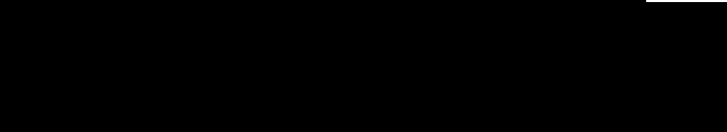
\includegraphics[width=0.9\textwidth]{pictures/primary}
\end{figure}

Natürlich kann jede der Vor- und Nachmethoden vorhanden sein oder nicht. Das einzige, was immer vorhanden sein muss, ist eine anwendbare Primärmethode. Außerdem haben Vor- und Nachmethoden weder Wissen von noch Einfluss auf das Ergebnis der Primärmethode. Sie eignen sich daher nur für Seiteneffekte. Dafür bieten sie der Klasse, die später erweitert wird, eine Möglichkeit, sicherzustellen, dass eine bestimmte Operation garantiert in allen Subklassen ausgeführt wird. Das kann zum Beispiel bei einer Methode zum Malen eines Bildes das Erstellen der Leinwand sein.

Zusätzlich zu Vor- und Nachmethoden gibt es noch Around-Methoden. Sie sind ähnlich zu einer Redefinition mit Super-Aufruf. Die Methode bestimmt selbst, ob und an welcher Stelle in ihrem Rumpf mit \texttt{call-next-method} (das CLOS-Äquivalent zu super) die nächste Methode aufegrufen werden soll. Die Aufrufreihenfolge ist wie folgt (vgl. \cite[S.103]{keene}):
\begin{itemize}
 \item CLOS ruft die spezifischste Around-Methode auf. Sie erhält die gleichen Parameter wie die generische Funktion bzw. Primärmethode.
 \item Falls eine Around-Methode \texttt{call-next-method} aufruft:
 \begin{itemize}
  \item Wenn es weitere anwendbare Around-Methoden gibt, wird die nächstspezifischste aufgerufen und das Ergebnis zurückgegeben.
  \item Ansonsten wird das komplette Framework aus Vor-, Primär- und Nachmethoden aufgerufen und das Ergebnis zurückgegeben.
 \end{itemize}
\end{itemize}

Ein Beispiel für eine Around-Methode ist das Messen der Zeit, die die Primärmethode benötigt. Da Around-Methoden eintscheiden können, \texttt{call-next-method} nicht aufzurufen, können sie den Aufruf aller Vor-, Nach- und Primärmethoden verhindern. Eine Around-Methode muss auch nicht das Ergebnis der Primärmethode zurückgeben (auch wenn es Konvention ist, das zu tun).

Wir haben damit gesehen, dass ein Umgang mit Mehrfachvererbung in CLOS sehr intuitiv und einfach bereitgestellt werden kann.

\section{Zwischenfazit}
Das Objektsystem von Racket bietet zwar Mixins und Traits, beide sind jedoch geschickt verpackte Einfachvererbung und werden sehr schnell sehr kompliziert, wenn die Anzahl an Klassen steigt und gleichbenannte Methoden und Felder vorkommen. CLOS hingegen bietet einen sehr intuitiven Umgang mit Mehrfachvererbung. Es gibt generische Methoden, Methodenkombination und Ergänzungsmethoden.

Da der Umgang mit Mehrfachvererbung, wie CLOS ihn bietet, auch im Objektsystem von Racket umgesetzt werden soll, schauen wir nun hinter die Kulissen. Zunächst wird die Implementation von CLOS beleuchtet und im Anschluss die Implementation des Racket-Objektsystems.

\chapter{Entwurf} 
Das Objektsystem von Racket soll um die Features Mehrfachvererbung, generische Methoden und Ergänzungsmethoden erweitert werden. Es werden dafür zunächst die Anforderungen an eine solche Umsetzung formuliert und anschließend einen Enwurf erarbeitet, der diese Anforderungen erfüllt. Es wird ein Vorschlag für die Erweiterung der Racket-Syntax um Mehrfachvererbung vorgestellt und Möglichkeiten der Einbindung in Racket diskutiert.

\section{Anforderungen}
Folgende Anforderungen sollen beachtet werden:
\begin{enumerate}
 \item Bestehender Code in Object-Racket funktioniert genauso wie vorher. Die Erweiterung soll keinen Einfluss auf bestehenden Racket-Code haben. Alle Funktionalität, die das Objektsystem zur Zeit bietet, soll auch nach Hinzufügen der Features auf dieselbe Art funktionieren und das gleiche Ergebnis liefern.
 \item Die Syntax passt sich in das Objektsystem von Racket ein. Neu hinzugefügte Makros und Funktionen sollen konsistent mit bestehenden Makros und Funktionen benannt werden und auf die gleiche Art und Weise aufrufbar sein. 
 \item Die Benutzung ist für jemanden, der CLOS kennt, intuitiv. Die definierten Makros und Funktionen sollen möglichst ähnlich zu benutzen sein wie in CLOS und das gleiche Verhalten zeigen (unter Beachtung von 2.).
\end{enumerate}

Die erste Anforderung soll gewährleisten, dass die entstehende Erweiterung auch in bestehenden Racket-Projekten eingebunden werden kann, ohne dass das die Funktionalität bestehender Klassen und Objekte beeinflusst. Die Erweiterung soll dazu ermuntern, Mehrfachvererbung zu nutzen an den Stellen, so es sinnvoll ist und das mit dem geringstmöglichen Änderungsaufwand. Es soll niemand gezwungen sein, alle bestehenden Klassen umzuschreiben, nur damit eine einzelne Klasse Mehrfachvererbung nutzen kann.

Die zweite Anforderung knüpft direkt an die erste an: Es ist einfacher, neue Funktionalität zu benutzen, wenn sie sehr ähnlich zu bereits bestehenden Konzepten ist. Für einen Entwickler, der sich bereits mit dem Objektsystem von Racket auskennt, soll die neue Funktionalität so intuitiv wie möglich sein. Dafür ist es ist beispielsweise hilfreich, wenn generische Funktionenen, die vom Konzept her sehr verwandt zu Methoden sind, auf eine ähnliche Weise benutzt werden können.

Die dritte Anforderung ist interessant für diejenigen, die beide Welten kennen: die von Racket und die von CLOS. Die Erweiterung integriert Bestandteile von CLOS in das Objektsystem von Racket. Dann sollten diese Bestandteile für jemanden, der CLOS kennt, leicht verständlich und möglichst ähnlich zu benutzen sein.

\section{Vorschlag für die Erweiterung von Racket}

\subsection{Mehrere Superklassen}
Für Mehrfachvererbung muss es zunächst möglich sein, mehrere Superklassen anzugeben. Analog zu CLOS soll dies in einer Liste möglich sein. Die Spezifikation der Superklassen als Liste ist jedoch lediglich eine Alternative, die direkte Angabe der Superklasse soll weiterhin möglich sein, um Anforderung 1 nicht zu verletzten. Wie in CLOS soll auch eine leere Liste angegeben werden können, in dem Fall wird automatisch die Rootklasse als Superklasse gesetzt. Da in CLOS die Liste nicht quotiert ist, soll auch in Racket auf Quotierung verzichtet werden. Die folgenden drei Aufrufe sollen zukünftig alle eine Klasse erzeugen, die \texttt{object\%} als (einzige) Superklasse hat (bisher ist in Racket nur die erste Form möglich):

\begin{lstlisting}
(class object% (super-new))
(class () (super-new))
(class (object%) (super-new))
\end{lstlisting}

In der Liste sollen auch mehrere Klassen angegeben werden können. Die Superklassen werden nach ihrer Präzedenz geordnet angegeben; diejenige mit der höchsten Präzedenz kommt zuerst, diejenige mit der niedrigsten Präzedenz zuletzt. 

\begin{lstlisting}
(class (my-class my-other-class ...) (super-new)) 
\end{lstlisting}

Die Funktion \texttt{super-new} sorgt dann dafür, dass die Konstruktoren aller angegebenen  Superklassen aufgerufen werden. Sie soll weiterhin an jeder Stelle in Rumpf der Klasse angegeben werden können. 

Gegebenenfalls ist auch eine alternative Definition mit Klassenparameter sinnvoll, sodass der Benutzer Kontrolle darüber hat, in welcher Reihenfolge die Konstruktoren der Superklasse aufgerufen werden. Dann muss jedoch auch mit dem Fall, dass der Benutzer nicht alle Superklassen aufruft, umgegangen werden -- beispielsweise durch Werfen eines Fehlers zur Auswertung oder beim Erstellen eines Objektes, oder durch automatisches Aufrufen aller fehlenden Superklassen am Ende des Rumpfes. Zudem muss abgewogen werden, ob diese Freiheit für den Benutzer die Implementierung nicht zu stark verkompliziert.

Falls mehr als eine Superklasse angegeben wird, so erbt die Klasse alle Felder und Methoden der beiden Oberklassen. Gibt es gleichbenannte Felder, so werden im Standardfall die Felder beziehungsweise Methoden der Klasse mit der höheren Präzedenz geerbt.

\subsection{Generische Funktionen}
Da Methoden im Objektsystem von Racket innerhalb von Klassen definiert werden, soll das auch für generische Funktionen gelten. Sie werden in der entsprechenden Oberklasse definiert. Für das attack-Beispiel aus der Racketeinführung wäre das die Klasse Thing. Methodendefinitionen starten in Racket mit \texttt{define/}, daher sollen generische Funktionen mit dem Schlüsselwort \texttt{define/generic} definiert werden. Die Syntax ist wie folgt:

\texttt{(define/generic ({\textless}function-name{\textgreater} {\textless}args{\textgreater}) {\textless}combination{\textgreater})}

Der Objekt-Parameter entfällt, da wir uns bereits in der Klasse, für die die Funktion spezialisiert ist, befinden. Subklassen können (müssen aber nicht) die generische Funktion durch eine öffentliche Methode implementieren. Für Klassen, die die Methode nicht explizit definieren, wird die Methode durch Methodenkombination erzeugt. Falls die Methodenkombination wegen fehlender Methoden fehlschlägt, gibt es wie in CLOS einen Laufzeitfehler.

Die in CLOS definierten Standardkombinationen sollen auch in Racket möglich sein: \texttt{+, min, max, list, append, begin, and, or}. 
Zusätzlich soll es möglich sein, eigene Kombinationen zu definieren.


\subsection{Vor- und Nachmethoden}
Vor- und Nachmethoden (und ggf. auch Around-Methoden) sollen auf ähnliche Weise über \texttt{define/before}, \texttt{define/after} beziehungsweise \texttt{define/around} definierbar sein. 

\texttt{(define/before ({\textless}method-name{\textgreater} {\textless}args{\textgreater}) {\textless}body{\textgreater})}\\
\texttt{(define/after ({\textless}method-name{\textgreater} {\textless}args{\textgreater}) {\textless}body{\textgreater})}\\
\texttt{(define/around ({\textless}method-name{\textgreater} {\textless}args{\textgreater}) {\textless}body{\textgreater})}

Der Methodenname muss mit einer in der Klasse sichtbaren Primärmethode übereinstimmen. Falls die Klasse keine entsprechende Primärmethode definiert oder erbt, so gibt es einen Laufzeitfehler.

\section{Einbindung in Racket}
Für die Einbindung in Racket gibt es drei Möglichkeiten:
\begin{enumerate}
 \item Ändern der Racket-Module, die an der Implementierung des Objektsystems beteiligt sind.
 \item Das Racket-Objektsystem als Blackbox betrachten und 
 \begin{enumerate}
  \item darauf aufbauend ein eigenes Objektssystem definieren.
  \item die Optionen, die an das \texttt{class}-Makro übergeben werden verändern und anschließend Racket die Objekterzeugung überlassen.
 \end{enumerate}
\end{enumerate}

Eine Veränderung der bestehenden Racket-Module hätte den Vorteil, dass wir direkten Zugriff auf alle Informationen, die zur Erzeugung der Klassen und Objekte von Racket verwendet werden, haben. Die Erzeugung von Klassen und Objekten kann direkt manipuliert werden und es ist vermutlich möglich wie in CLOS Instanzen von Methoden zu erzeugen und diese dann in einer festgelegten Reihenfolge auszuführen. 

Dafür ist jedoch ein sehr tiefgehehendes Verständnis der Racket-Implementierung notwendig. Leider ist diese kaum dokumentiert. Das Modul, das beispielsweise für die Expansion des \texttt{class}-Makros zuständig ist, heißt \texttt{class-internal} und befindet sich in \texttt{racket/collects/racket/private}. Allein die Definition des \texttt{class}-makros erstreckt sich über fast 1400 Zeilen und es ist nicht ungewöhnlich, über 100 Codezeilen keinen Kommentar anzutreffen. Das Objektsystem von Racket ist sehr umfangreich; es gibt unzählige Klassenoptionen und sie alle müssen in dem Makro abgedeckt werden. Allein die Stellen zu finden, die für eine Erweiterung des Objektsystems angepasst werden müssten, würde bereits einen erheblichen Anteil der Bearbeitungszeit ausmachen.

Eine direkte Veränderung des Objektsystems erschwert außerdem das Ziel, dass bestehende Objektsysteme genauso wie vorher funktionieren sollen. Die Seiteneffekte von Änderungen sind nur schwer abzuschätzen und ein Test der kompletten Funktionalität von Racket ist im Rahmen dieser Arbeit nicht möglich. Zudem ist diese Lösung nur schwer wartbar: Der Code wäre verteilt über die komplette Implementierung von Object-Racket. 

Durch das Betrachten von Object-Racket als Blackbox würde die Verständlichkeit von Zusammenhängen und die Wartbarkeit stark erhöht. Die Erweiterung befindet sich in einem einzelnen (oder wenigen) Modul und kann daher leicht im Rahmen eines Übungsbetriebs verwendet und eingebunden werden.

Der Nachteil ist, dass es dann keinen Zugriff auf die Implementierungsdetails von Racket gibt. Wissen über die Klassenhierarchie oder darüber, welche Felder und Methoden eine Klasse definiert, müssen wir selbst bereitstellen. Die Zeit, die aufgewendet werden muss um diese Informationen festzuhalten, wird jedoch deutlich geringer eingeschätzt als der Aufwand, die bestehende Racket-Implementierung in vollem Umfang zu verstehen. 

Die Entscheidung fällt deshalb auf Option 2.

Auf Racket aufbauend ein eigenes Objektsystem zu definieren (2a) ist sehr nah an der Idee, die in AMOP verfolgt wird. Es gibt uns die volle Kontrolle über das Verhalten von Vererbung und Objekten und bietet daher eine einfache Möglichkeit, beispielsweise Methodenkombination umzusetzen. Den vollen Umfang der Funktionalität von Object-Racket anzubieten bedeutet dann jedoch, dass jede Klassenoption und jedes Verhalten, das diese Optionen bewirkt, 1:1 nachgebaut werden oder zumindest an die der Implementation zugrundeliegenden Racket-Objekte weitergeleitet werden müsste.

Die Tatsache, dass ein eigenes Objektsystem definiert wird, hat auch den Nachteil, dass wir nun zwei Objetsysteme haben: das von Object-Racket und das darauf aufbaunde und von uns definierte. Beide sind jedoch nicht miteinander kompatibel. Über Objekte, die in Object-Racket erzeugt wurden, haben wir keine Informationen; wir kennen nicht die Vererbungshierarchie, vorhandene Felder oder Methoden. 

Das bedeutet, dass Objekte in Modulen, die das von uns definierte Objektsystem nutzen, nicht mit Objekten in Modulen kommunizieren könnten, die es nicht benutzen. Sobald ein Modul eines bestehendes Racket-System das erweiterte Objektsystem nutzt, müssten alle Module es benutzen. Das steht im Widerspruch zu der Anforderung, dass bestehende Racket-Implementationen durch das Benutzen der Erweiterung nicht beeinflusst werden sollen.

Option 2b, eine simple Veränderung der Klassenoptionen, die an das Makro übergeben werden, löst all diese Probleme, stellt uns jedoch vor eine andere Herausforderung: Mehrfachvererbung und Methodenkombination rein auf Syntaxebene zu implementieren. Wir können keine Felder oder Methoden definieren und auswerten; die Erzeugung all dieser Dinge übernimmt Object-Racket schließlich für uns. Das heißt, allein anhand der Sytax, die wir in das \texttt{class}-Makro injizieren (oder daraus entfernen), muss Mehrfachvererbung erreicht werden.

Die Vor- und Nachteile der drei Optionen sind noch einmal in Tabelle \ref{einbindung} zusammengefasst.

\begin{table}[h]
\centering
\begin{tabular}{|l|c|c|c|}
 \hline
 & \textbf{1} & \textbf{2a} & \textbf{2b}\\\hline
 Direkter Zugriff auf Implemtierungsdetails   & \cmark & \cmark & \xmark \\\hline
 Angemessener Zeitaufwand                     & \xmark & \cmark & \cmark \\\hline
 Gute Wartbarkeit                             & \xmark & \cmark & \cmark \\\hline 
 Bestehende Objektsysteme bleiben unverändert & \xmark & \xmark & \cmark \\\hline
\end{tabular}
\caption{Vergleich der drei Ansätze zur Einbindung in Racket.}
\label{einbindung}
\end{table}

Da wir auf die Anforderung, dass bestehende Objektsysteme unverändert funktionieren sollen, nicht verzichten wollen, wird im Folgenden Option 2b umgesetzt: eine reine Veränderung der Optionen, die an das \texttt{class}-Makro übergeben werden.


% -----------------------------------------------------------------------------------------

\chapter{Makros} 
\label{makros}
Um die Implementation einer Sprache zu verstehen, zu verändern oder zu erweitern ist es unumlässlich, sich mit Makros auseinanderzusetzen. 

Vorgehen... % TODO

Dieses Kapitel basiert auf dem Guide ``Fear of Macros'' von Greg Hendershott \cite{fearofmacros} und dem Racket-Guide für Makros \cite{racketguide-macros}. Die Code-Beispiele in ``Fear of Macros'' sind sehr anschaulich und wurden für diese Arbeit nahezu unverändert übernommen.


\section{Transformers}
\subsection{Was ist ein Syntaxtransformer?}

Ein Makro ist im Grunde eine Funktion. Sie erhält ein Stück Syntax als Eingabe und gibt ein anderes Stück Syntax zurück. Sie \textit{transformiert} Syntax. Wir können einen solchen Syntax-Transformer mit \texttt{define-syntax} definieren:

\begin{lstlisting}
(define-syntax foo
  (lambda (stx)
    (syntax "I am foo")))
\end{lstlisting}

Ein Aufruf von foo ergibt dann:

\begin{lstlisting}
> (foo)
\end{lstlisting}
{\routput {\qq}I am foo{\qq}}

Durch die Verwendung von \texttt{define-syntax} geschieht eine Transformer-Bindung. Wir teilen dem Racket-Compiler mit: ``Wann immer du im Quelltext ein Stück Syntax findest, das mit \texttt{foo} startet, gib es an meine Transformer-Funktion und ersetze es mit der Syntax, die ich dir zurück gebe.'' Racket gibt also alles, das aussieht wie \texttt{(foo ...)} an unsere Funktion und wir können neue Syntax zurückgeben, die stattdessen verwendet wird, ähnlich zu einer Suchen-und-Ersetzen-Operation.

\begin{lstlisting}
> (foo 1 2 3)
\end{lstlisting}
{\routput ``I am foo''}

Analog zu der Kurzschreibweise \texttt{(define (f x) ...)} anstelle von \texttt{(define (lambda (x) ...)} gibt es auch eine Kurzschreibweise für \texttt{define-syntax}:

\begin{lstlisting}
(define-syntax (also-foo stx)
  (syntax "I am also foo"))
  
> (also-foo)
\end{lstlisting}
{\routput ``I am also foo''}

Und auch für \texttt{syntax} gibt es die Abkürzung \texttt{\#\q} (analog zu \texttt{\q} und \texttt{quote}):

\begin{lstlisting}
(define-syntax (quoted-foo stx)
  #'"I am also foo, using #' instead of syntax")
  
> (also-foo)
\end{lstlisting}
{\routput {\qq}I am also foo, using \#\q instead of syntax{\qq}}

Obwohl sich die Funktion nun nicht mehr stark von einem \texttt{define} unterscheidet, ist es immer noch eine Transformer-Funktion, die Syntax entgegennimmt und Syntax zurückgibt.

\subsection{Syntax-Objekte}
Bisher haben wir die Eingabe-Syntax einfach ignoriert und eine festgelegte Syntax zurückgegen. Übsicherweise soll jedoch die Eingabe-Syntax transformiert werden. Wenn wir Syntax definieren, erhalten wir ein Syntax-Objekt:

\begin{lstlisting}
(define stx #'(+ 1 (* 2 3)))

> stx
\end{lstlisting}
{\routput\#<syntax:2:14 (+ 1 (* 2 3))>}

Ein Syntaxobjekt besteht aus einer Repräsentation des Ausdrucks, enthält aber auch Informationen über die Datei, Zeile und Spalte in der es definiert wurde sowie den Sichtbarkeitsbereich von Variablen (\emph{lexical scope}). All diese Informationen kann man mit entsprechenden Funktionen abfragen. Zwei dieser Funktionen, die auf Syntax arbeiten, sind \texttt{syntax->datum} und \texttt{syntax-e}. 

\texttt{syntax->datum} wandelt die Syntax in einen quotierten Racket-Ausdruck um:

\begin{lstlisting}
> (syntax->datum stx)
\end{lstlisting}
{\rsymbol (+ 1 (* 2 3))}

Analog lässt sich mit \texttt{datum->syntax} aus einem quotierten Racket-Ausdruck ein Syntax-Objekt erzeugen. Die Funktion benötigt zusätzlich zu der Syntax noch einen Kontext. Üblicherweise genügt es, als Kontext das ursprüngliche Syntaxobjekt anzugeben.

\texttt{syntax-e} geht nur ein Level tief. Es kann eine Liste von Syntax-Objekten zurückgeben:

\begin{lstlisting}
> (syntax-e lst)
\end{lstlisting}
{\rsymbol (\#<syntax:2:15 +> \#<syntax:2:17 1> \#<syntax:2:19 (* 2 3)>)}

Jedes dieser Syntax-Objekte kann dann rekursiv mit \texttt{sytax-e} weiter aufgelöst werden. Genau das macht \texttt{syntax->datum}.

Beim Transformieren von Syntax nehmen wir üblicherweise die Bestandteile der Syntax, die uns gegeben wird, ändern ihre Reihenfolge, ersetzen einige von ihnen oder führen gänzlich neue Bestandteile ein.

\subsection{Transformieren von Syntax}

Ein simples Beispiel, das die Reihenfolge der Syntax umkehrt:

\begin{lstlisting}
(define-syntax (reverse-me stx)
  (datum->syntax stx (reverse (cdr (syntax->datum stx)))))
  
> (reverse-me "backwards" "am" "I" values)
\end{lstlisting}
{\routput {\qq}I{\qq} {\qq}am{\qq} {\qq}backwards{\qq}}

Die Transformer-Funktion erhält die Syntax \texttt{\#\q(reverse-me {\qq}backwards{\qq} {\qq}am{\qq} {\qq}I{\qq} values)}. Zuerst wird diese durch \texttt{syntax->datum} in einen quotierten Ausdruck umgewandelt. Mit \texttt{cdr} entfernen wir das erste Element (reverse-me) aus der Liste, geben diese als Parameter als \texttt{reverse} und erhalten die Liste \texttt{\q(values {\qq}I{\qq} {\qq}am{\qq} {\qq}backwards{\qq})}. Durch Übergeben an die Funktion \texttt{datum->syntax} erhalten wir daraus ein Syntax-Objekt. Dieses Objekt wird von der Transformer-Funktion zurückgegeben und diese Syntax wird anschließend vom Compiler ausgewertet.

Der Syntax-Transformer wird zur Übersetzungszeit ausgewertet. Das bedeutet, dass die Teilstücke der Syntax zwar verschoben und ersetzt werden -- aber nicht ausgewertet. Das geschieht erst zur Laufzeit. Dadurch ermöglichen uns Makros beispielsweise die Definition eines eigenen \texttt{if} durch Benutzen von \texttt{cond}.

Würden wir \texttt{if} als normale Racket-Funtion definieren, so würden alle Parameter ausgewertet, bevor sie überhaupt an die Funktion gegeben werden. Das wird spätestens dann sichtbar, wenn sie Seiteneffekte beinhalten oder in einem Zweig der Fallunterscheidung ein rekursiver Aufruf steckt. Durch die Definition als Makro haben wir die Möglichkeit das \texttt{if} bereits zur Übersetzungszeit durch ein \texttt{cond} zu ersetzten:

\begin{lstlisting}
(define-syntax (my-if stx)
  (let ((xs (cdr (syntax->datum stx))))
    (datum->syntax stx `(cond [,(car xs) ,(cadr xs)]
                              [else ,(caddr xs)]))))
\end{lstlisting}

Durch das Quasiquote \texttt{`} werden nur die mit Komma markierten Teile der Liste ausgewertet.

Eine Liste immer mit \texttt{car}, \texttt{cadr} und so weiter zu zerlegen ist jedoch sehr anstrengend zu fehleranfällig. Eleganter geht es mithilfe von Pattern-Matching. Racket bietet dafür die Funktion \texttt{match}. 

Unsere Transformer-Funktion wird zur Übersetzungszeit ausgewertet. Zu diesem Zeitpunkt wird jedoch nur \texttt{racket/base} automatisch zur Verfügung gestellt, nicht das komplette \texttt{racket}. Alle Funktionen, die wir darüber hinaus benutzen wollen, müssen wir mit per Hand anfordern -- un zwar zur Übersetzungszeit. Dafür gibt es die \texttt{for-syntax}-Option von \texttt{require}:

\begin{lstlisting}
(require (for-syntax racket/match))

(define-syntax (my-if-using-match stx)
  (match (syntax-e stx)
    [(list name condition true-expr false-expr)
     (datum->syntax stx `(cond [,condition ,true-expr]
                               [else ,false-expr]))]))
\end{lstlisting}

\subsection{Hilfsfunktionen}
Wenn wir eine Hilfsfunktion für unser Makro benötigen, können wir sie nicht einfach mit \texttt{define} definieren und benutzen -- die Definition würde zur Laufzeit existieren, aber wir brauchen sie zur Übersetzungszeit. Eine Möglichkeit ist es, die Funktion in ein anderes Modul zu schreiben und dieses mit \texttt{for-syntax} einzubinden.

Falls wir die Funktion stattdessen im selben Modul definieren wollen, können wir sie innerhalb eines \texttt{begin-for-syntax}-Blocks definieren oder alternativ die Kurzform \texttt{define-for-syntax} benutzen:

\begin{lstlisting}
(begin-for-syntax
  (define (my-helper-function ...) 
    ...))
  
(define-for-syntax (my-helper-function ...)
  ...)
\end{lstlisting}

\section{Pattern Matching}
\subsection{define-syntax und syntax-case}
Das Makrosystem von Racket bietet eine noch bequemere Funktion für Pattern Matching: \texttt{syntax-case}.

Anstatt

\begin{lstlisting}
(require (for-syntax racket/match))
(define-syntax (my-if-using-match stx)
  (match (syntax-e stx)
    [(list name condition true-expr false-expr)
     (datum->syntax stx `(cond [,condition ,true-expr]
                               [else ,false-expr]))]))
\end{lstlisting}

können wir schreiben:

\begin{lstlisting}
(define-syntax (my-if-using-syntax-case stx)
  (syntax-case stx ()
    [(_ condition true-expr false-expr)
      #'(cond [condition true-expr]
             [else false-expr])]))
\end{lstlisting}

Das Quasiquote ist nicht mehr nötig und auch \texttt{datum->syntax} entfällt. Stattdessen stellen wir ein Template bereit, welches Variablen aus dem Pattern benutzt. 

\subsection{define-syntax-rule}

Auch für \texttt{syntax-case} gibt es eine Kurzform für einfache Pattern-Matching-Fälle namens \texttt{define-syntax-rule}:

\begin{lstlisting}
(define-syntax-rule 
  (my-if-using-syntax-rule condition true-expr false-expr) ; Pattern
  (cond [condition true-expr]                              ; Template
        [else false-expr]))
\end{lstlisting}

Diese Definition sieht so einfach aus, dass man denken könnte, es wäre eine normale Laufzeit-Funktion -- aber sie ist es nicht. Sie läuft zur Übersetzungszeit, nicht zur Laufzeit. 

\subsection{Sichtbarkeit von Variablen}

Sehr komfortable an dem Makro ist, dass es die Sichbarkeit von Variablen berücksichtigt. Nehmen wir beispielsweise das Makro, das zwei Werte vertauscht (nach \cite{racketguide-macros}):

\begin{lstlisting}
(define-syntax-rule (swap x y)
  (let ([tmp x])
    (set! x y)
    (set! y tmp)))
\end{lstlisting}

Angenommen, in der lokalen Umgebung des Makroaufrufs gibt es bereits eine Variable namens \texttt{tmp}:

\begin{lstlisting}
(let ([tmp 1]
      [other 2])
  (swap tmp other)
  (list tmp other))
\end{lstlisting}

Würden wir dahergehen und das Makro naiv expandieren, so würden die Werte nicht vertauscht werden:

\begin{lstlisting}
(let ([tmp 1]         ; tmp1
      [other 2])
  (let ([tmp tmp])    ; tmp2 verschattet tmp1
    (set! tmp other)  ; tmp2 = 2
    (set! other tmp)) ; other = tmp2 = 2
  (list tmp other))   ; (tmp1, other)
\end{lstlisting}

Tatsächlich produziert Racket jedoch nicht die naive Expansion. Sobald Variablen im lokalen Kontext des Makroaufrufs mit Makro-Variablen übereinstimmen, werden die Variablen im Makro vor der Expansion umbenannt. Wir erhalten also:

\begin{lstlisting}
(let ([tmp 1]
      [other 2])
  (let ([tmp_1 tmp])
    (set! tmp other)
    (set! other tmp_1))
  (list tmp other))
\end{lstlisting}

mit dem korrekten Ergebnis \texttt{(2,1)}.

\subsection{syntax-rules}
\texttt{define-syntax-rule} bindet ein Makro, das ein einzelnes Pattern abgleicht. Racket's Makro-System unterstützt mit \texttt{syntax-rules} jedoch auch Transformer für mehrere Patterns, die mit dem gleichen Bezeichner starten.

Beispielsweise könnten wir ein Makro definieren, das sowohl zwei als auch drei Werte miteinander vertauschen kann (nach \cite{racketguide-macros}):

\begin{lstlisting}
(define-syntax rotate
  (syntax-rules ()
    [(rotate a b) (swap a b)]
    [(rotate a b c) (begin
                     (swap a b)
                     (swap b c))]))
\end{lstlisting}

Es ist sogar möglich, Patterns beliebiger Länge in einem Makro zu matchen. Für eine beliebige Anzahl an Parametern können wir einfach \texttt{...} schreiben. Das Makro ähnelt dann einer rekursiven Funktion mit einem Standardfall (oder mehr) und einer Regel, wie mit dem Rest der Parameter zu verfahren ist (nach \cite{racketguide-macros}):

\begin{lstlisting}
(define-syntax rotate
  (syntax-rules ()
    [(rotate a) (void)]
    [(rotate a b c ...) (begin
                          (swap a b)
                          (rotate b c ...))]))
\end{lstlisting}

% \subsection{with-syntax}
% In einem Template können bisher nur Werte ersetzt werden, die vorher im Pattern bereits aufgetaucht sind. Oft wollen wir jedoch neue Teile definieren und benutzten. Das geht, indem \texttt{syntax-case} ineinander verschachtelt wird. Eine besser lesbare Kurzform für das Einführen einer neuen Pattern-Variable ist \texttt{with-syntax}. Es kann ähnlich wie ein \texttt{let} benutzt werden:

\section{Fehlerbehandlung}
Genau wie mit Standard-Funktionen gibt es auch bei Makros verschiedene Möglichkeiten mit einem fehlerhaftem Aufruf umzugehen: Ignorieren, Schreiben von fehlerbehandelndem Code oder \texttt{syntax-parse}. 

\texttt{syntax-parse} erlaubt es uns, das Eingabe-Pattern auf Richtigkeit zu prüfen, ähnlich zu einer Typprüfung oder einem Vertrag.

http://docs.racket-lang.org/syntax/stxparse.html %TODO

% -----------------------------------------------------------------------------------------

\chapter{CLOS: Backstage}
% \section{Das Objektsystem von Racket: Backstage}
\label{cpl}


\chapter{Implementation}  % überwiegend eigener Teil

\chapter{Analyse/Erprobung/Auswertung/Test}

\chapter{Zusammenfassung und Ausblick}

% -----------------------------------------------------------------------------------------

\appendix
\chapter{Anhang}
\section{Beispiel Object-Racket}
\label{or-example}
\lstinputlisting{code/object-racket-example.rkt}

\section{Beispiel CLOS}
\label{clos-example}
\lstinputlisting{code/clos-example.rkt}
\phantomsection % benötigt für korrekte pdf-darstellung
\addcontentsline{toc}{chapter}{Literaturverzeichnis}
\bibliographystyle{alpha} % originally: natbib % Din 1505 nach Lorenzen (Das konkrete Aussehen des Litverzeichnisses ist im header festgelegt)
% \bibliography{bibliography/literatur}  % Pfad zur *.bib-Datei (Dateiendung wird weggelassen)
%TODO korrekt zitieren
Werden noch korrekt zitiert und ggf. durch bessere Quellen ersetzt. 
\begin{thebibliography}{}
 \bibitem{amop} The Art of the Metaobject Protocol 
 \bibitem{racketguide-dialects} \url{http://docs.racket-lang.org/guide/dialects.html}
 \bibitem{neu-edu} \url{http://www.ccs.neu.edu/home/matthias/Thoughts/Programming\_with\_Class\_in\_Racket.html}
 \bibitem{neu-edu2} \url{http://www.ccs.neu.edu/home/matthias/Tmp/Class/programming-with-class/Classes\_in\_Racket.html}
 \bibitem{racketguide-classes} Racket Guide: 13. Classes and Objects \url{https://docs.racket-lang.org/guide/classes.html}
 \bibitem{racketref-classes} Racket Reference: 6. Classes and Objects \url{https://docs.racket-lang.org/reference/mzlib\_class.html}
 \bibitem{racketguide-macros} \url{https://docs.racket-lang.org/guide/macros.html}
 \bibitem{racketref-macros} \url{https://docs.racket-lang.org/reference/Macros.html}
 \bibitem{fearofmacros} \url{http://www.greghendershott.com/fear-of-macros/index.html}
 \bibitem{keene} Sonya E. Keene, ``Object-Oriented Programming in Common Lisp. A Programmer's Guide to CLOS''
\end{thebibliography}

\cleardoublepage % TODO
\backmatter 

\thispagestyle{empty}

\vspace*{\fill}
\pagestyle{empty}

{\normalsize
\begin{center}\textbf{Eidesstattliche Erklärung}\end{center}
Hiermit versichere ich an Eides statt, dass ich die vorliegende Arbeit im Masterstudiengang Informatik selbstständig verfasst und keine anderen als die angegebenen Hilfsmittel – insbesondere keine im Quellenverzeichnis nicht benannten Internet-Quellen – benutzt habe. Alle Stellen, die wörtlich oder sinngemäß aus Veröffentlichungen entnommen wurden, sind als solche kenntlich gemacht. Ich versichere weiterhin, dass ich die Arbeit vorher nicht in einem anderen Prüfungsverfahren eingereicht habe und die eingereichte schriftliche Fassung der auf dem elektronischen Speichermedium entspricht.
\vspace*{1cm}\\
Hamburg, den XX.XX.20XX
\hspace*{\fill}\begin{tabular}{@{}l@{}}\hline
\makebox[5cm]{Vorname Nachname}
\end{tabular}
\vspace*{3cm}
%Dies ist optional, ggf. löschen!
\begin{center}\textbf{Veröffentlichung}\end{center}
Ich stimme der Einstellung der Arbeit in die Bibliothek des Fachbereichs Informatik zu.
\vspace*{1cm}\\
Hamburg, den XX.XX.20XX
\hspace*{\fill}\begin{tabular}{@{}l@{}}\hline
\makebox[5cm]{Vorname Nachname}
\end{tabular}
}
\vspace*{\fill} 

\end{document}
